\documentclass[14pt]{beamer}
\usepackage[T2A]{fontenc}
\usepackage[utf8]{inputenc}
\usepackage[english,russian]{babel}
\usepackage{amssymb,amsfonts,amsmath,mathtext}
\usepackage{cite,enumerate,float,indentfirst}

\graphicspath{{../images/}{images/}} 

\usepackage{../Dissertation/phdstyle}
%\usepackage[edges]{forest}
\usepgfplotslibrary{fillbetween}
%\newcommand{\W}{\Omega}
\newcommand{\Wedm}{\W^{edm}}
\newcommand{\Wmdm}{\W^{mdm}}
%\newcommand{\gef}{\gamma_{eff}}

%\usepackage{animate}
%\usepackage{tcolorbox}

% \usetheme[secheader]{Boadilla}
% \usecolortheme{seahorse}

%\usetheme{Pittsburgh}
%\usecolortheme{whale}

\usetheme{Boadilla}

\beamertemplatenavigationsymbolsempty

\newcommand{\todo}{\alert}
%%% Основные сведения %%%
\newcommand{\thesisAuthorLastName}{\todo{Аксентьев}}
\newcommand{\thesisAuthorOtherNames}{\todo{Александр Евгеньевич}}
\newcommand{\thesisAuthorInitials}{\todo{А.\,Е.}}
\newcommand{\thesisAuthor}             % Диссертация, ФИО автора
{%
    \texorpdfstring{% \texorpdfstring takes two arguments and uses the first for (La)TeX and the second for pdf
        \thesisAuthorLastName~\thesisAuthorOtherNames% так будет отображаться на титульном листе или в тексте, где будет использоваться переменная
    }{%
        \thesisAuthorLastName, \thesisAuthorOtherNames% эта запись для свойств pdf-файла. В таком виде, если pdf будет обработан программами для сбора библиографических сведений, будет правильно представлена фамилия.
    }
}
\newcommand{\thesisAuthorShort}        % Диссертация, ФИО автора инициалами
{\thesisAuthorInitials~\thesisAuthorLastName}
%\newcommand{\thesisUdk}                % Диссертация, УДК
%{\todo{xxx.xxx}}
\newcommand{\thesisTitle}              % Диссертация, название
{\todo{Метод замороженного спина  для поиска электрического дипольного момента дейтрона в накопительном кольце}}
\newcommand{\thesisSpecialtyNumber}    % Диссертация, специальность, номер
{\todo{01.04.01}}
\newcommand{\thesisSpecialtyTitle}     % Диссертация, специальность, название
{\todo{Приборы и методы экспериментальной физики}}
\newcommand{\thesisDegree}             % Диссертация, ученая степень
{\todo{кандидата физико-математических наук}}
\newcommand{\thesisDegreeShort}        % Диссертация, ученая степень, краткая запись
{\todo{канд. физ.-мат. наук}}
\newcommand{\thesisCity}               % Диссертация, город написания диссертации
{\todo{Москва}}
\newcommand{\thesisYear}               % Диссертация, год написания диссертации
{\todo{2019}}
\newcommand{\thesisOrganization}       % Диссертация, организация
{\todo{Национальный Ядерный Исследовательский Университет ``МИФИ'' \\ (НИЯУ МИФИ)}}
\newcommand{\thesisOrganizationShort}  % Диссертация, краткое название организации для доклада
{\todo{НазУчДисРаб}}

\newcommand{\thesisInOrganization}     % Диссертация, организация в предложном падеже: Работа выполнена в ...
{\todo{учреждении, в~котором выполнялась данная диссертационная работа}}

\newcommand{\supervisorFio}            % Научный руководитель, ФИО
{\todo{Сеничев Юрий Валериевич}}
\newcommand{\supervisorRegalia}        % Научный руководитель, регалии
{\todo{д.ф.-.м.н., проф.}}
\newcommand{\supervisorFioShort}       % Научный руководитель, ФИО
{\todo{Ю.\,В.~Сеничев}}
\newcommand{\supervisorRegaliaShort}   % Научный руководитель, регалии
{\todo{уч.~ст.,~уч.~зв.}}


\newcommand{\opponentOneFio}           % Оппонент 1, ФИО
{\todo{Фамилия Имя Отчество}}
\newcommand{\opponentOneRegalia}       % Оппонент 1, регалии
{\todo{доктор физико-математических наук, профессор}}
\newcommand{\opponentOneJobPlace}      % Оппонент 1, место работы
{\todo{Не очень длинное название для места работы}}
\newcommand{\opponentOneJobPost}       % Оппонент 1, должность
{\todo{старший научный сотрудник}}

\newcommand{\opponentTwoFio}           % Оппонент 2, ФИО
{\todo{Фамилия Имя Отчество}}
\newcommand{\opponentTwoRegalia}       % Оппонент 2, регалии
{\todo{кандидат физико-математических наук}}
\newcommand{\opponentTwoJobPlace}      % Оппонент 2, место работы
{\todo{Основное место работы c длинным длинным длинным длинным названием}}
\newcommand{\opponentTwoJobPost}       % Оппонент 2, должность
{\todo{старший научный сотрудник}}

\newcommand{\leadingOrganizationTitle} % Ведущая организация, дополнительные строки
{\todo{Федеральное государственное бюджетное образовательное учреждение высшего профессионального образования с~длинным длинным длинным длинным названием}}

\newcommand{\defenseDate}              % Защита, дата
{\todo{DD mmmmmmmm YYYY~г.~в~XX часов}}
\newcommand{\defenseCouncilNumber}     % Защита, номер диссертационного совета
{\todo{Д\,123.456.78}}
\newcommand{\defenseCouncilTitle}      % Защита, учреждение диссертационного совета
{\todo{Название учреждения}}
\newcommand{\defenseCouncilAddress}    % Защита, адрес учреждение диссертационного совета
{\todo{Адрес}}
\newcommand{\defenseCouncilPhone}      % Телефон для справок
{\todo{+7~(0000)~00-00-00}}

\newcommand{\defenseSecretaryFio}      % Секретарь диссертационного совета, ФИО
{\todo{Фамилия Имя Отчество}}
\newcommand{\defenseSecretaryRegalia}  % Секретарь диссертационного совета, регалии
{\todo{д-р~физ.-мат. наук}}            % Для сокращений есть ГОСТы, например: ГОСТ Р 7.0.12-2011 + http://base.garant.ru/179724/#block_30000

\newcommand{\synopsisLibrary}          % Автореферат, название библиотеки
{\todo{Название библиотеки}}
\newcommand{\synopsisDate}             % Автореферат, дата рассылки
{\todo{DD mmmmmmmm YYYY года}}

% To avoid conflict with beamer class use \providecommand
\providecommand{\keywords}%            % Ключевые слова для метаданных PDF диссертации и автореферата
{}
      % Основные сведения
\renewcommand{\todo}[1]{\textcolor{black}{#1}}

\setbeamercolor{footline}{fg=blue}
\setbeamertemplate{footline}{
  \leavevmode%
  \hbox{%
  \begin{beamercolorbox}[wd=.333333\paperwidth,ht=2.25ex,dp=1ex,center]{}%
    % И. О. Фамилия, Организация кратко
    \thesisAuthorShort, \thesisOrganizationShort
  \end{beamercolorbox}%
  \begin{beamercolorbox}[wd=.333333\paperwidth,ht=2.25ex,dp=1ex,center]{}%
    % Город, 20XX
    \thesisCity, \thesisYear
  \end{beamercolorbox}%
  \begin{beamercolorbox}[wd=.333333\paperwidth,ht=2.25ex,dp=1ex,right]{}%
  Стр. \insertframenumber{} из \inserttotalframenumber \hspace*{2ex}
  \end{beamercolorbox}}%
  \vskip0pt%
}

\newcommand{\itemi}{\item[\checkmark]}

%%\title{\small{Название презентации}}
%\title{\small{\thesisTitle}}
%\author{\small{%
%\emph{Выступающий:}~\thesisAuthorShort\\%
%\emph{Руководитель:}~\supervisorARegaliaShort~\supervisorAFioShort
%}\\%
%\vspace{30pt}%
%\thesisOrganization%
%\vspace{20pt}%
%}
%\date{\small{\thesisCity, \thesisYear}}

\begin{document}
	\title{\small{\textcolor{blue}{\thesisTitle}}}
	\author{\small{%
			\begin{tabular}{lll}
				\emph{Соискатель:} & & \thesisAuthorShort\\
				\emph{Руководитель:} & \supervisorARegaliaShort & \supervisorAFioShort \\
				\emph{Консультант:} & \supervisorBRegaliaShort & \supervisorBFioShort
			\end{tabular}
		}\\%
		\vspace{30pt}%
		\thesisOrganization%
		\vspace{20pt}%
	}
	\date{\small{\thesisCity, \thesisYear}}

\maketitle

\section{Формальности}
%%%%%%%%%%%%%%%%%%%%%%%%%%%%%%%%%%%%%%%%%%%%%%%%%%%%%%%%%%%%%%%%%%%%%%%%%%%%%%%%%%%%%%%%%%%%%%%%%%%%
%\begin{frame}{Актуальность}
%	\framesubtitle{Зачем нужно искать ЭДМ?}
%	\begin{itemize}[<+->]
%		\item Вопрос: Барионная асимметрия вселенной
%		\item Ответ: нарушение СР-симметрии, как одно из условий бариогенеза
%		\item Существование перманентного ЭДМ нарушает СР-симметрию
%		\item Стандартная Модель предсказывает ЭДМ $<10^{-31}~e\cdot cm$
%		\item[$\Rightarrow$] Обнаружение большего ЭДМ --- свидетельство физики за гранью СМ
%	\end{itemize}
%\end{frame}
\begin{frame}{Актуальность}
	\begin{center}
		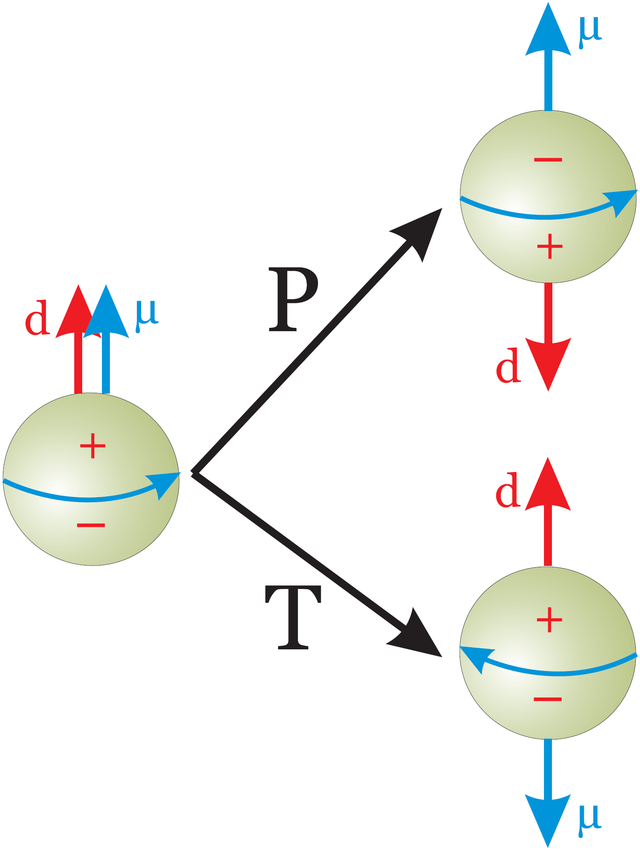
\includegraphics[height=.8\paperheight]{NEDM_P&T_violation}
	\end{center}
\end{frame}

\begin{frame}{Цель исследования}
%\begin{block}{}
Разработка метода поиска электрического дипольного момента частицы в накопительном кольце, 
позволяющего достичь точность $10^{-29}$\ecm.
%\end{block}
\end{frame}
\begin{frame}{Задачи исследования}
	\begin{itemize}
		\item Разработать метод измерения ЭДМ дейтрона на основе измерений частоты прецессии спина в накопительном кольце.
		\item Проанализировать требования к магнитооптической структуре кольца-накопителя для поиска ЭДМ.
		\item Исследовать спин-декогеренцию пучка дейтронов в окрестности состояния ``замороженного спина.''
	\end{itemize}
\end{frame}
\begin{frame}
	\begin{itemize} 
		\item Исследовать влияние несовершенств оптической структуры кольца на спин-орбитальную динамику. 
		\item Промоделировать процедуру калибровки нормализованной частоты прецессии спина (спин-тюна) при смене полярности ведущего поля.
		\item Изучить статистические свойства метода измерения электрического дипольного момента.
	\end{itemize}
\end{frame}

\begin{frame}{Научная новизна}
	\begin{enumerate}
		\item Предложен метод измерения ЭДМ дейтрона,
		основанный исключительно на измерении частоты прецессии спина в накопительном кольце 
		с ограничением по точности, оцениваемым на уровне $10^{-29}$~\ecm.
		\item Изучена спин-орбитальная динамика дейтронного пучка в окрестности состояния ``замороженного спина.'' 
	\end{enumerate}
\end{frame}
\begin{frame}
	\begin{enumerate} \setcounter{enumi}{2}
		\item Предложен метод калибровки среднего по пучку спин-тюна, позволяющий уменьшить вклад систематических ошибок.
		\item Введено определение эффективного значения фактора Лоренца, необходимое для 
		определения зависимости спин-тюна частицы от её координат в фазовом пространстве. 
		\item Сделаны статистические оценки предельной чувствительности измерения ЭДМ предложенным методом.
	\end{enumerate}
\end{frame}

\begin{frame}{Практическая значимость}
	Разработанный метод представляет интерес с точки зрения планирования экспериментов по поиску ЭДМ
	на различных ускорителях, в том числе на ускорительном комплексе NICA ОИЯИ (Дубна).
\end{frame}

\begin{frame}{Апробация}
	\begin{itemize}
		\item Во время исследований по оптимизации времени когерентности спина при помощи секступольных полей на ускорительном комплексе COSY (Исследовательский центр ``Юлих'').
		\item Результаты работы вошли в подготавливаемый коллаборацией CPEDM для CERN отчёта, под названием ``Feasibility study for an EDM Storage Ring.''
		\item Основные результаты работы докладывались на международных концеренциях IPAC'17, IPAC'19, LaPlas III--V, а также конференциях коллаборации JEDI, и семинарах IKP-2 Forschungszentrum J\"ulich.
	\end{itemize}
\end{frame}

%\begin{frame}{Структура диссертации}
%	Диссертация состоит из \textbf{четырёх} глав:
%	\begin{enumerate}
%		\item посвящена анализу методологии измерения электрического дипольного момента (ЭДМ) 
%		элементарой частицы при помощи накопительного кольца, работающего в режиме ``замороженного спина'': 
%		\begin{itemize}
%			\item вводится понятие ``замороженного спина'';
%			\item анализируются основные предложения по методу измерения ЭДМ, систематизируются их проблемы, предлагается новый метод;
%			\item представлены три варианта магнитооптической структуры напокительного кольца для измерения дейтрона предложенным методом.
%		\end{itemize}
%	\end{enumerate}
%\end{frame}
%\begin{frame}
%	\begin{enumerate}\setcounter{enumi}{1}
%			\item посвящена анализу проблем измерения ЭДМ частицы 
%			в накопительном кольце с замороженным спином и поиску их решений:
%			\begin{itemize}
%				\item возмущения спиновой динамики частицы;
%				\item спин-декогеренция частиц пучка в окрестности состояния ``замороженного спина'';
%				\item свойства МДМ компоненты частоты спин-прецесии -- основной систематической ошибкой измерений;
%				\item смена полярности ведущего поля ускорителя.
%			\end{itemize}
%		\item посвящена статистическому моделированию эксперимента 
%		и оценке его возможной статистической точности:
%		\begin{itemize}
%			\item исследуется возможность повышения эффективности
%			поляриметрии путём использования частотно-модулированной схемы выборки;
%			\item процедура обработки данных поляриметрии протестирована на модельных данных.
%		\end{itemize}
%	\end{enumerate}
%\end{frame}
%\begin{frame}
%	\begin{columns}
%		\begin{column}{.55\linewidth}
%			\includegraphics[width=\linewidth]{COSY_Facility}
%		\end{column}
%		\begin{column}{.5\linewidth}
%			\begin{enumerate}\setcounter{enumi}{3}
%				\item описаны наиболее значимые (для данной работы) технологии, 
%				разработанные в рамках исследований, проведённых на синхротроне COSY:
%				\begin{itemize}
%					\item высокоточное измерение частоты прецесии спина;% (с точностью до $10^{-10}$ в измерительном цикле 100~секунд);
%					\item юстировка квадруполей при помощи пучка;% (Beam Based Alignment~\cite{Wagner:BBA2018});
%					\item оптимизация времени когерентности спина.%~\cite{COSY:SCT:IPAC15, Guidoboni:STORI14}.
%				\end{itemize}
%			\end{enumerate}
%		\end{column}
%	\end{columns}
%\end{frame}

\section{Краткое  введение в область}
%%%%%%%%%%%%%%%%%%%%%%%%%%%%%%%%%%%%%%%%%%%%%%%%%%%%%%%%%%%%%%%%%%%%%%%%%%%%%%%%%%%%%%
%\begin{frame}{Методы поиска ЭДМ}
%	\begin{forest}
%		[Накопительное кольцо
%		[Замороженный\\ спин, align=center
%		[Измерения\\ амплитуды, align=center
%		[BNL FS]
%		[D-MR]
%		]
%		[Измерения\\ частоты, align=center
%		[SW]
%		[FDM]
%		]
%		]
%		[Незамороженный\\ спин, align=center
%		[Частично-\\замороженный\\спин\\(ВЧ Вин-фильтр), align=center]
%		]
%		]
%	\end{forest}
%\end{frame}



%\begin{frame}{Варианты структур}
%\framesubtitle{Истинно-замороженный спин}
%\centering
%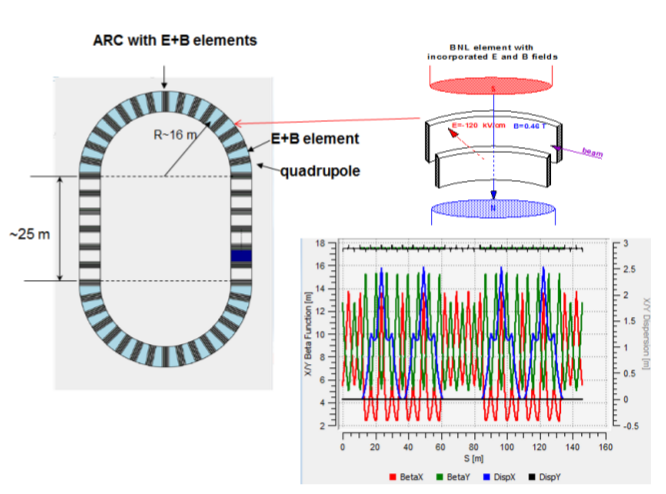
\includegraphics[width=.8\linewidth]{chapter2/BNL_lattice}
%\end{frame}
%
%\begin{frame}{Варианты структур}
%\framesubtitle{Квази-замороженный спин}
%\centering
%\begin{tikzpicture}
%\node (SX) {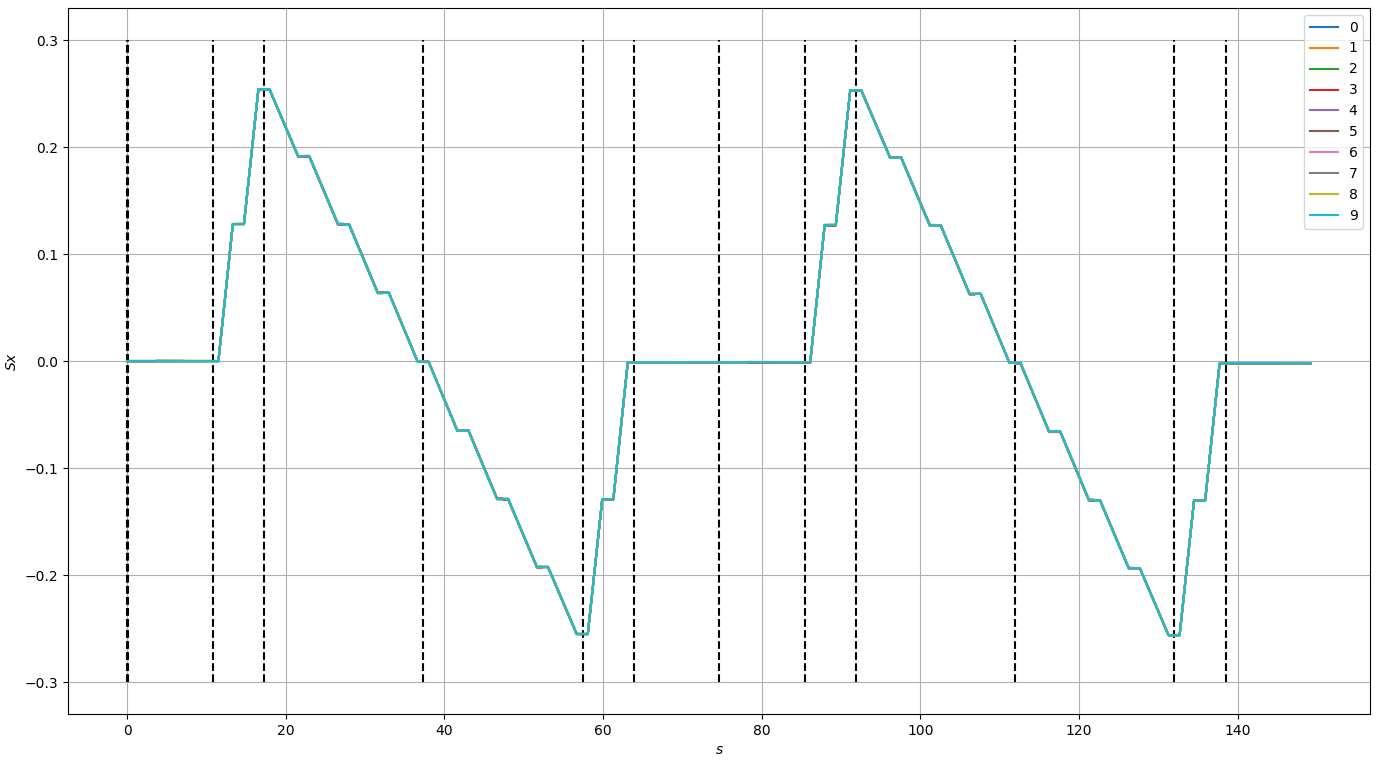
\includegraphics[width=\linewidth]{chapter2/EB_QFS_Sx_vs_s_1turn}};
%\pause
%\node (form) at (SX.north east) [xshift=-2cm, yshift=.5cm] {$J_0(\Phi_s) \approx 1 - \frac{\Phi_s^2}{4}$};
%\pause
%\node (6_3) at (SX.center)[xshift=-2cm, yshift=2cm]
%{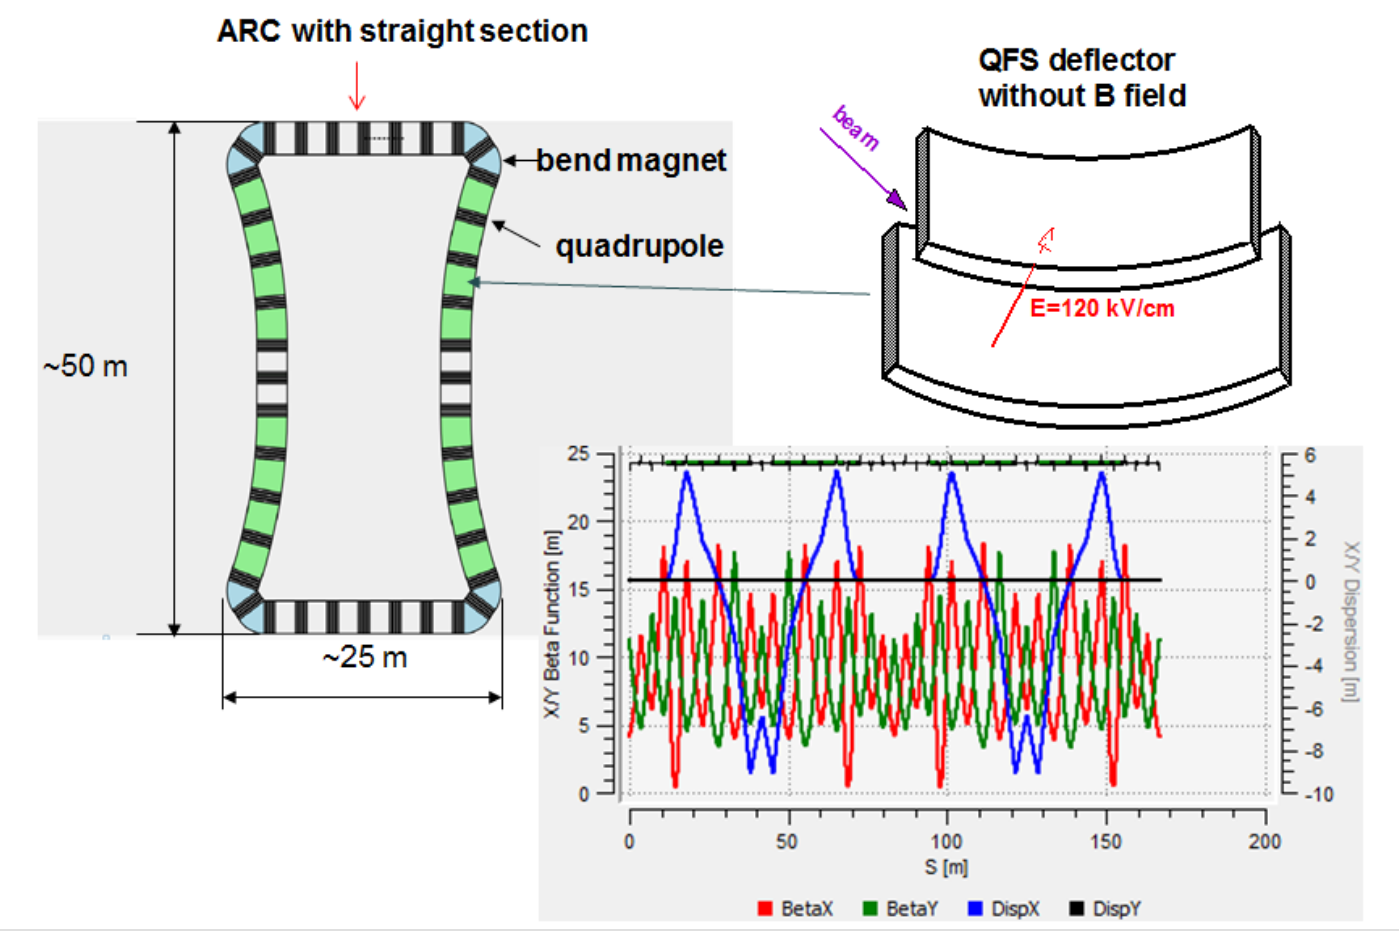
\includegraphics[width=.7\linewidth]{chapter2/6_3_lattice}};
%\pause
%\node (EB) at (SX.center)[xshift=2cm, yshift=-.07cm]
%{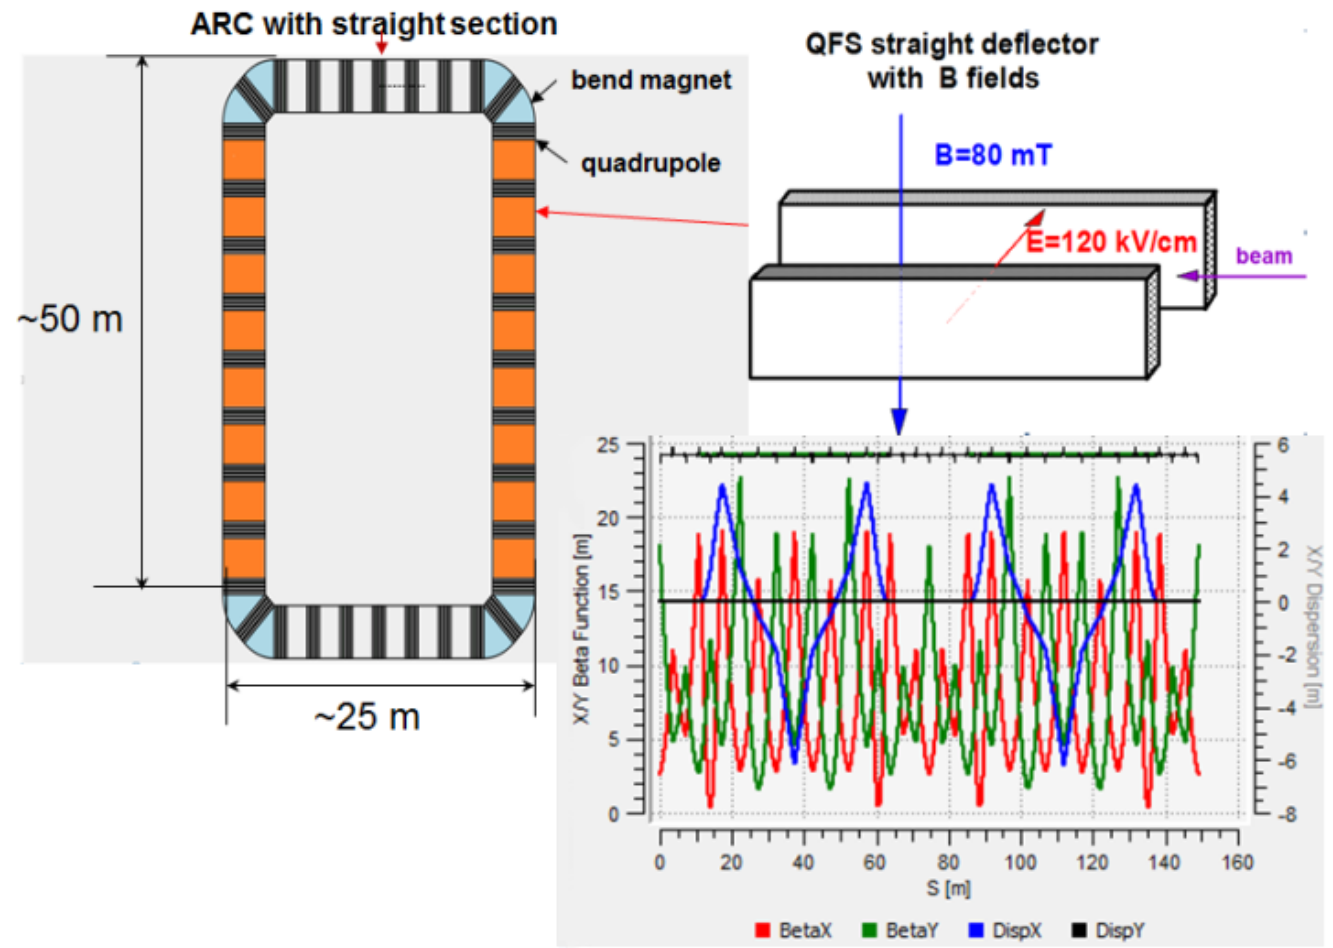
\includegraphics[width=.7\linewidth]{chapter2/E+B_lattice}};
%\end{tikzpicture}
%\end{frame}

%\begin{frame}{Измерение амплитуды vs частоты}
%\[
%P_y = A\cdot \sin\Big[\underbrace{\sqrt{(\w_{edm} + \w_{imp})^2 + \w_y^2 + \w_z^2}}_{\W}\cdot t + \delta\Big]
%\]
%\begin{itemize}
%	\item \textbf{Амплитуда:} 
%	\begin{itemize}
%		\item Останавливаем МДМ-прецессию и в \textbf{горизонтальной}, и в \textbf{вертикальной} плоскости
%		\item Наблюдаем за изменением \textbf{пространственной ориентации} вектора поляризации пучка
%	\end{itemize}
%	\item \textbf{Частота:}
%	\begin{itemize}
%		\item Останавливаем МДМ-прецессию \textbf{только} в горизонтальной плоскости
%		\item Наблюдаем за изменением в \textbf{угловой скорости} прецессии поляризации в вертикальной плоскости
%	\end{itemize}
%\end{itemize}
%\end{frame}
%
%\begin{frame}{Достоинства частотного метода}
%\begin{itemize}
%\item Менее жёсткие условия на точность установки элементов (не нужно исключать МДМ-вращение в вертикальной плоскости)
%\item Устойчивое состояние \textbf{двумерно}-замороженного спина (решает проблему геометрической фазы)
%\item Проще в отношении поляриметрии
%\end{itemize}
%\end{frame}

\section{Экспериментальная база и метод исследования}
%%%%%%%%%%%%%%%%%%%%%%%%%%%%%%%%%%%%%%%%%%%%%%%%%%%%%%%%%%%%%%%%%%%%%%%%%%%%%%%%%%%%%%%%%%%%%%%%%%%%%%%
\begin{frame}{COSY как инструмент для поиска ЭДМ}
	\begin{columns}
		\column{.55\linewidth}
		\centering
		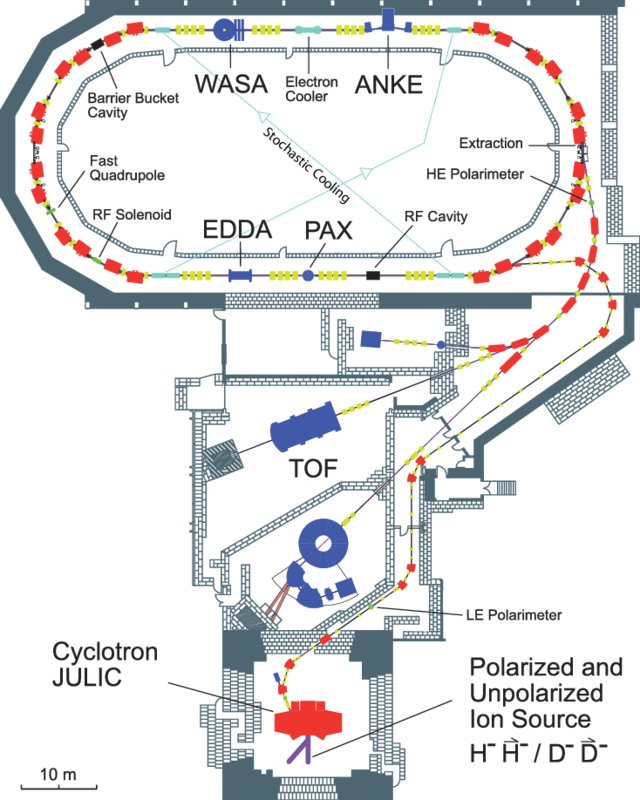
\includegraphics[width=\linewidth]{COSY_facility}
		\column{.5\linewidth}
		\begin{itemize}
			\item[$-$] Чисто магнитное кольцо
			\item[$+$] Источник поляризованных H$^-$/D$^-$
			\item[$+$] Циклотрон JULIC
			\item[$+$] Кольцо COSY 184~м
			\item[$+$] Внутренняя/внешняя мишени
			\item[$+$] Два вида охлаждения
		\end{itemize}
	\end{columns}
	
\end{frame}
\begin{frame}{Код COSY Infinity}
	% Здесь про то, как Кози вычисляет трансфер матрицы
	\begin{itemize}
		\item Разработка М. Берца и К. Макино (Michigan State University).
		\item Основан на дифференциальной алгебре; позволяет вычислять трансфер-матрицы элементов до (потенциально) любого порядка разложения ряда Тэйлора.
		\item Трекинговый код, учитывающий спиновую динамику.
	\end{itemize}
\end{frame}
\begin{frame}{Спин-трекинг в COSY Infinity} 
	%З десь про то, что строятся орбитальная и и спин трансфер-матрицы, и что Т-БМТ в
	% спин трансфер матрице
	\[
	\begin{cases}
	\vec{z}_n &= \mathcal{M}(\vec{z}_{n-1}), \\
	\vec{S}_n &= \hat A(\vec z_{n-1})\cdot \vec S_{n-1}
	\end{cases}
	\]
\end{frame}

\section{Содержание диссертации}
%%%%%%%%%%%%%%%%%%%%%%%%%%%%%%%%%%%%%%%%%%%%%%%%%%%%%%%%%%%%%%%%%%%%%%%%%%%%%%%%%%%%%%%%%%%%%%%%%%%%%%%%
\begin{frame}{Принцип измерения ЭДМ методом ``замороженного спина''}
	\begin{block}{Уравнение Томаса-БМТ}
		$\frac{\rd \vec s}{\rd t} = \vec s \times \bkt{\underbrace{a_0\cdot\vec B + a_1\cdot\vec E\times\vec\beta}_{\vec\Wmdm} + \underbrace{b_0\cdot\vec E + b_1\cdot\vec\beta\times\vec B}_{\vec\Wedm}}$
	\end{block}
	\begin{block}{Замороженный спин}
		$\Wmdm_{(y)} = 0$
	\end{block}
\end{frame}

\begin{frame}{Схема ускорителя}
	\centering
	\begin{tikzpicture}
	\node (scheme) {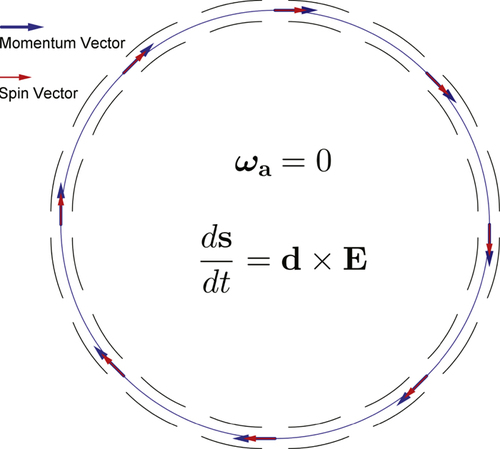
\includegraphics[width=.7\linewidth]{FS_ring}}; % из Proton EDM proposal
	\pause
	\node (real) at (scheme.center){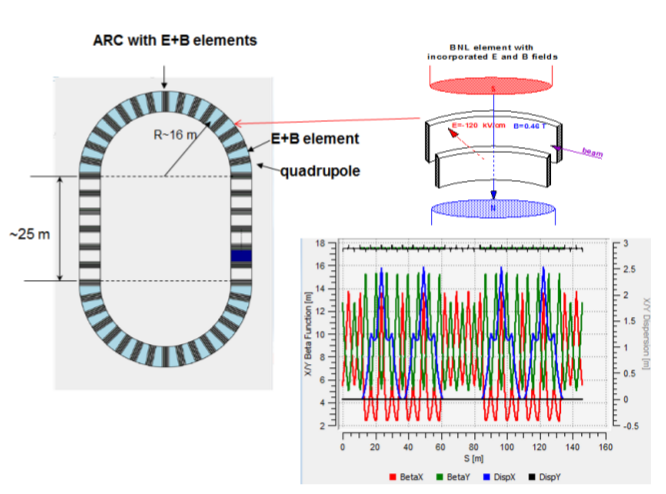
\includegraphics[width=.9\linewidth]{chapter2/BNL_lattice}};
%	\pause
%	\node (QFS1) at (real.center)[xshift=-3cm, yshift=-2cm]{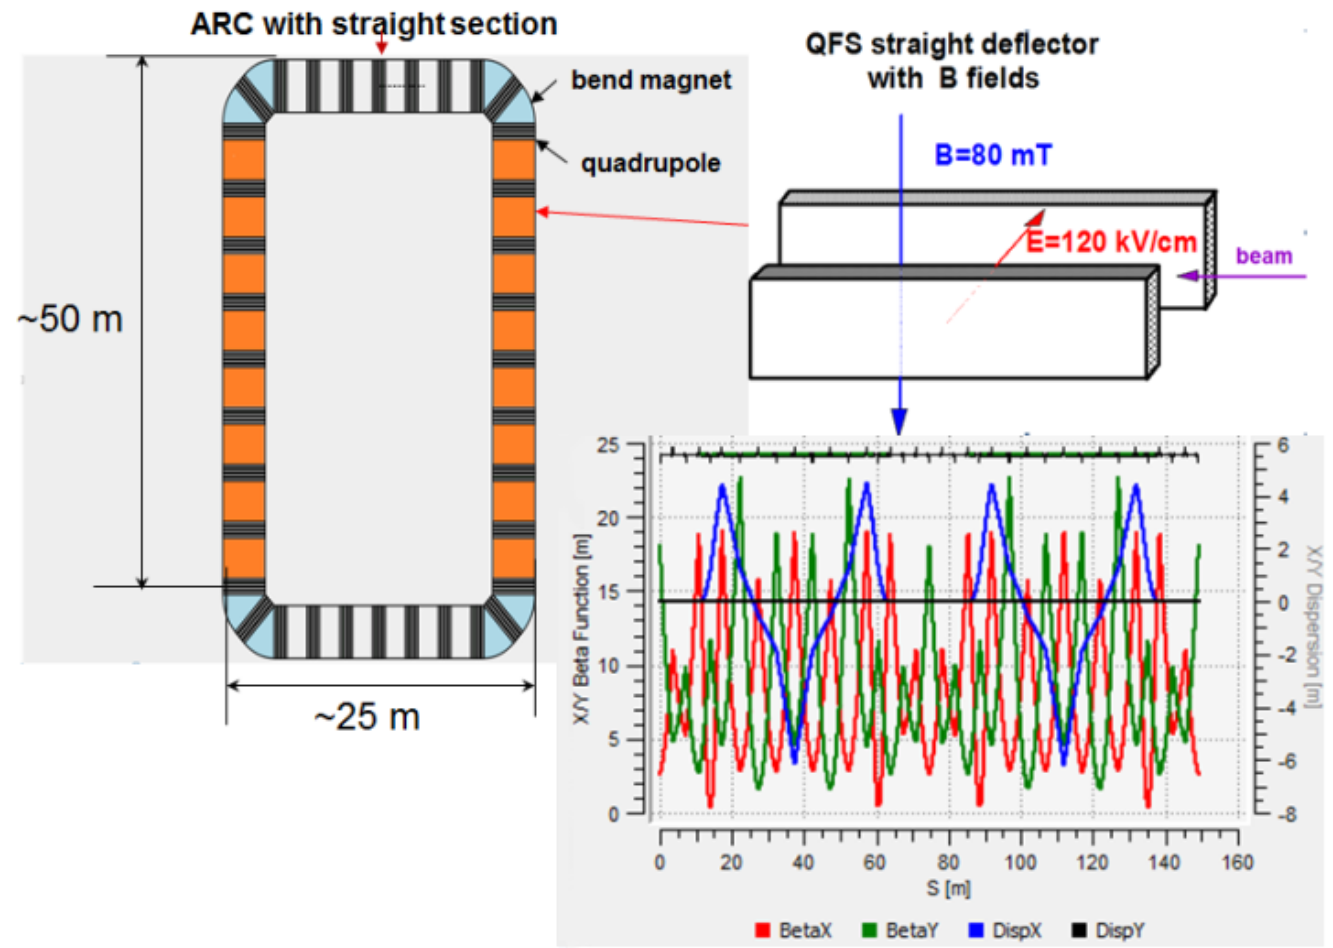
\includegraphics[width=.6\linewidth]{chapter2/E+B_lattice}};
%	\pause 
%	\node (QFS2) at (real.center)[xshift=2cm, yshift=-2cm]{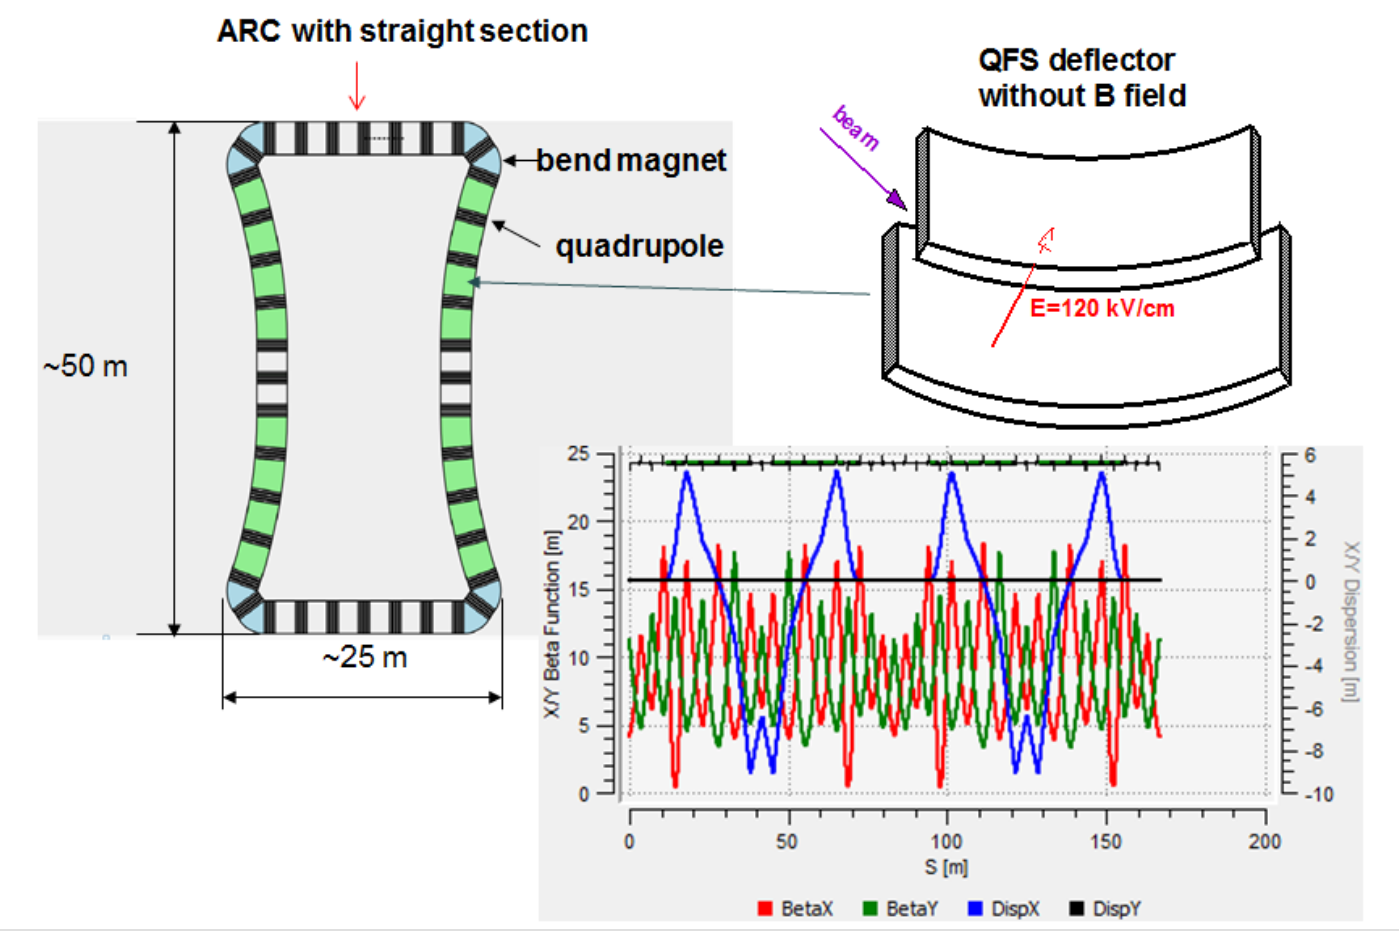
\includegraphics[width=.6\linewidth]{chapter2/6_3_lattice}};
	\end{tikzpicture}
\end{frame}

\begin{frame}{Общие проблемы поиска ЭДМ в накопительном кольце}
	\begin{enumerate}
		\item Возмущения спиновой динамики, связанные с бетатронными колебаниями частиц.
		\item Спин-декогеренция частиц пучка в окрестности состояния ``замороженного спина.''
		\item МДМ-компонента спин-прецессии, связанная с неидеальностями оптической структуры ускорителя.
		\item Смена полярности ведущего поля, требуемая для сокращения в конечном выражении оценки ЭДМ МДМ-компоненты частоты спин-прецессии.
	\end{enumerate}
\end{frame}

\begin{frame}{Возмущения спин-динамики}
	\begin{block}{Проблема}
		Вариация амплитуды фитируемого сигнала
	\end{block}
	\begin{block}{Выводы}
		Возмущения амплитуды сигнала
		\begin{itemize}
			\item на два порядка меньше случайной ошибки поляриметрии;
			\item влияют на оценку частоты с коэффициентом аттеньюации 10;
			\item поддаются контролю при использовании частотного подхода к измерениям.
		\end{itemize}
	\end{block}
\end{frame}
\begin{frame}{Спин-декогеренция}\centering
	\begin{block}{Проблема}
		Ограничение на длительность измерительного цикла
	\end{block}
\begin{columns}
	\begin{column}{.5\linewidth}
		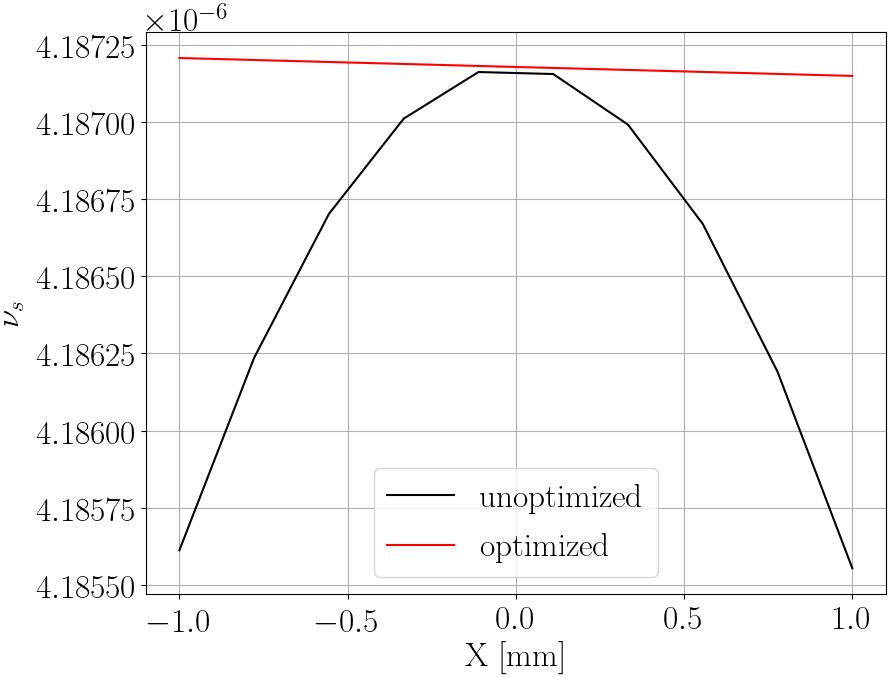
\includegraphics[width=\linewidth]{decoh_sim/spin_tune_decoh_x_offset}
	\end{column}
	\begin{column}{.5\linewidth}
		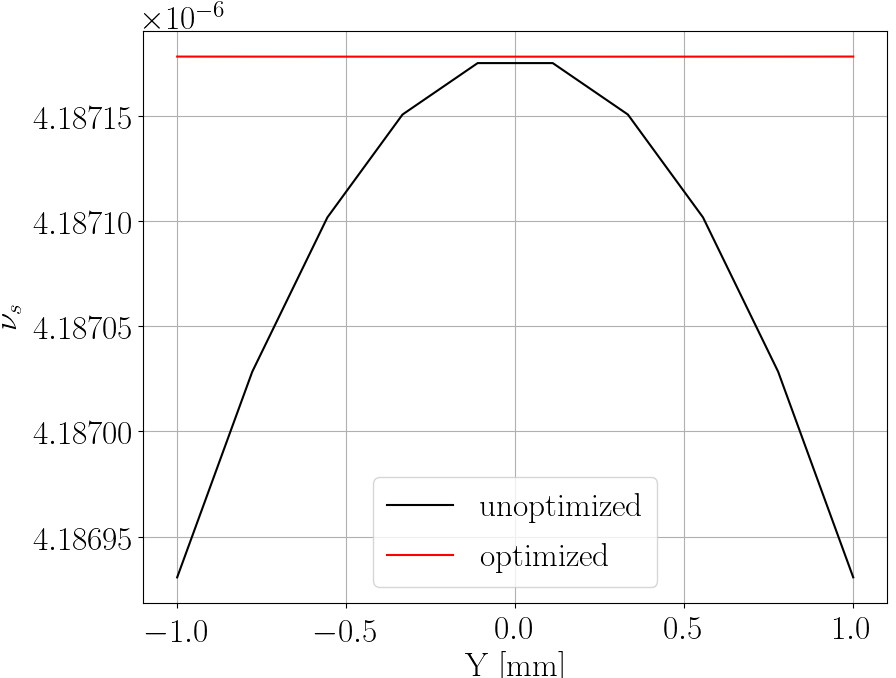
\includegraphics[width=\linewidth]{decoh_sim/spin_tune_decoh_y_offset}
	\end{column}
\end{columns}
%	\begin{block}{Выводы}
%		\begin{enumerate}
%			\item В частотных методах измерения ЭДМ спин-декогеренция переходит из плоскости замкнутой орбиты, в плоскость измерения поляризации.
%			\item Секступольные элементы одновременно выравнивают как \textbf{частоты}, так и \textbf{направления} осей прецессии спинов частиц.
%		\end{enumerate}
%	\end{block}
\end{frame}
\begin{frame}{МДМ-компонента спин-прецессии}
	\begin{block}{Проблема}
		Основная систематическая ошибка $\Wmdm$
	\end{block}
\begin{columns}
	\begin{column}{.5\linewidth}\centering
		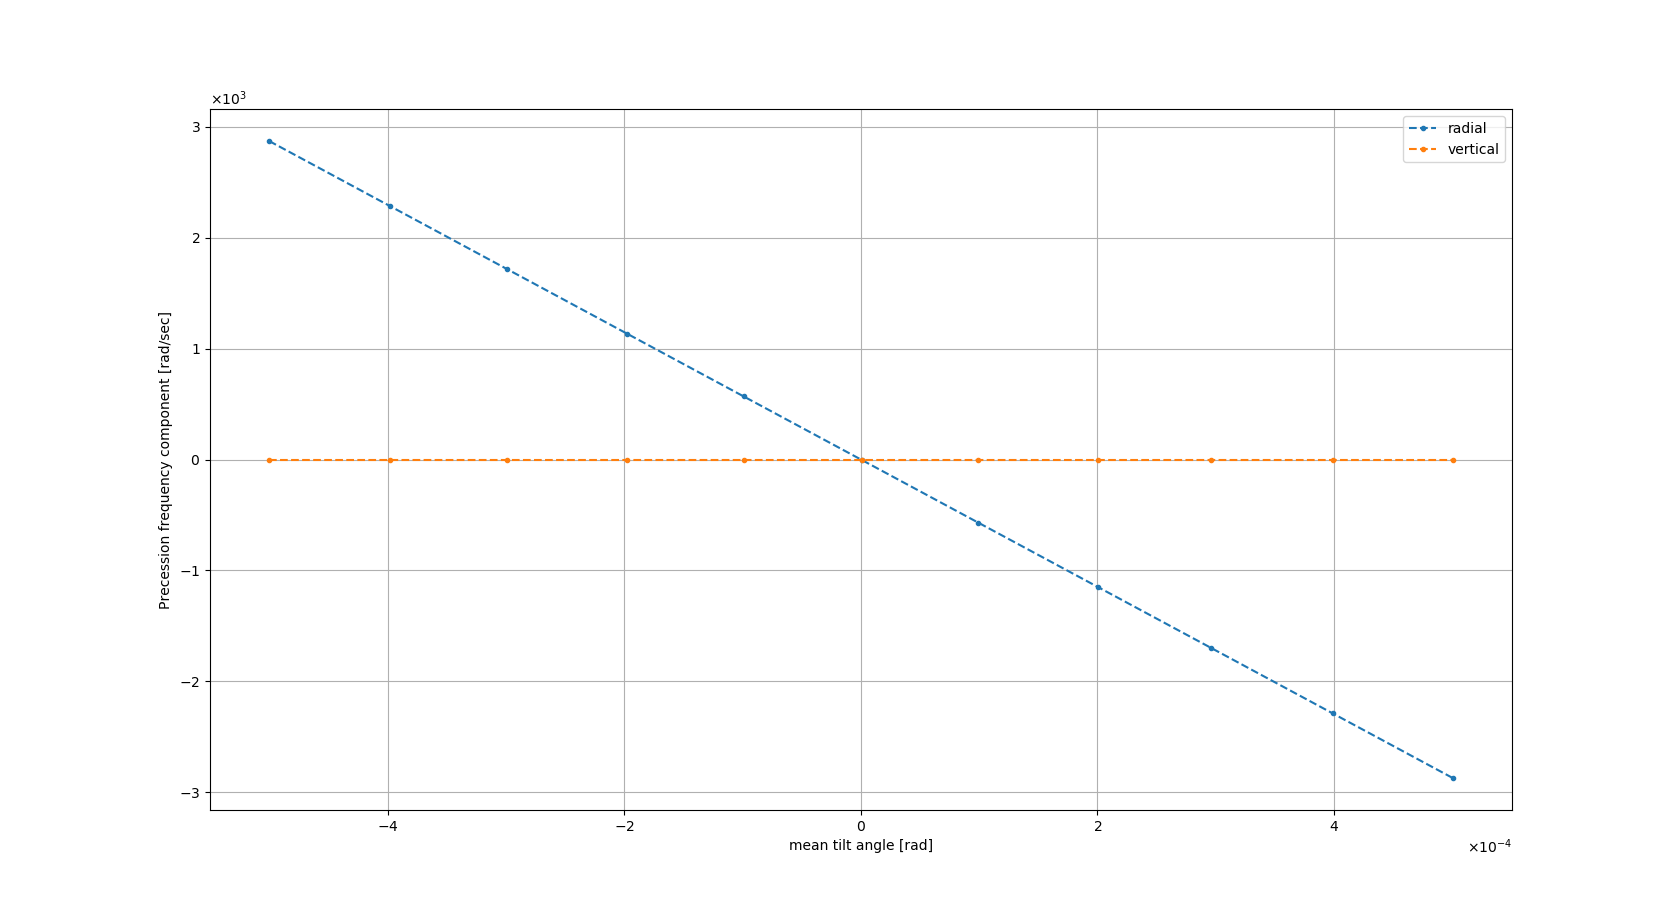
\includegraphics[width=\linewidth]{fake_signal_sim/linearity_test_shifting_gauss_freq}
		$\Wmdm = L(\avg{\theta_{tilt}})$
	\end{column}
	\begin{column}{.5\linewidth}\centering
		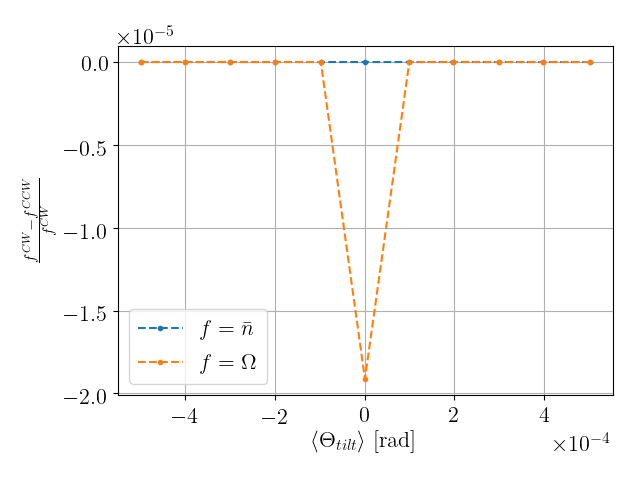
\includegraphics[width=\linewidth]{fake_signal_sim/linearity_test_shifting_gauss_rel_diff}
		$\Wmdm_{CW} \approx \Wmdm_{CCW}$
	\end{column}
\end{columns}
%	\begin{block}{Выводы}
%		\begin{enumerate}
%			\item Зависит только от \textbf{среднего} угла наклона $\avg{\theta_{tilt}}$, но не от конкретной последовательности наклонов оптических элементов ускорителя.
%			\item Зависимость носит линейный характер: $\Wmdm = L(\avg{\theta_{tilt}})$.
%			\item Устраняется в статистике путём измерений частоты прецесии спина в противоположно движущемся пучке.
%		\end{enumerate}
%	\end{block}
\end{frame}
\begin{frame}{Смена полярности ведущего поля}\centering
	\begin{block}{Проблема}
		Сменить полярность поля таким образом, чтобы воспроизвести величину $\Wmdm_x$ во всех измерительных циклах с точностью не хуже $10^{-7}$~рад/сек
	\end{block}
		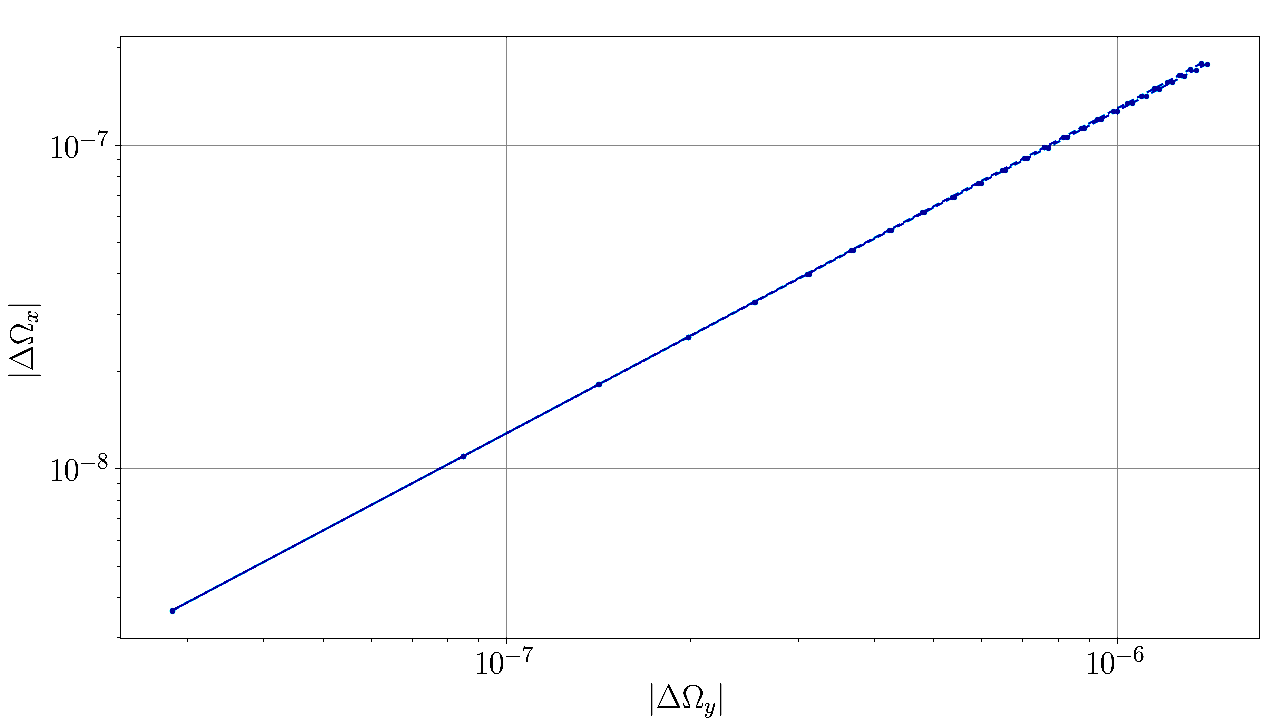
\includegraphics[width=.7\linewidth]{GFF/GFF_omegas_range_Y}
%	\begin{block}{Выводы}
%		\begin{enumerate}
%			\item Воспроизведение величины магнитного поля не достаточно; необходимо восстанавливать эффективный Лоренц-фактор центра масс пучка.
%			\item Если $|\Delta\Wmdm_y| < 10^{-7}$~рад/сек, то $|\Delta\Wmdm_x|<10^{-7}$~рад/сек.
%		\end{enumerate}
%	\end{block}
\end{frame}

\begin{frame}{Статистическое моделирование}
	\begin{block}{Выводы}
		\centering
		\begin{tabular}{rrr}
			\hline
			Инфо. (\%$\mathrm{FI_{tot}}$) & Длительность ($\times\tau_d$) & Сигнал/шум  \\
			\hline
			95            & 3.0                     & 0.4         \\
			90            & 2.3                     & 1.1         \\
			70            & 1.2                     & 5.5         \\
			50            & 0.7                     & 11.7        \\
			\hline
		\end{tabular}
	\begin{enumerate}
		\item Полезная длительность измерительного цикла не превосходит $3\cdot\tau_d$.
		\item За один измерительный цикл в 1~000~сек можно достичь $\sigma_{\hat\w}\approx 10^{-7}$~рад/сек, что за год измерений позволяет оценить ЭДМ с точностью $10^{-29}$\ecm.
	\end{enumerate}
	\end{block} 
\end{frame}

\begin{frame}{Результаты на COSY}
	\begin{block}{Успехи}
		\begin{enumerate}
			\item Высокоточное измерение нормализованной частоты прецессии спина: $\sigma_{\nu_s}\approx 10^{-10}$, $\sigma_{edm}\approx 10^{-24}$\ecm.
			\item Юстировка квадруполей с помощью пучка: точность определения положения квадруполей до 0.2~мм.
			\item Оптимизация времени когерентности спина: время жизни поляризации свыше 1~000~сек.
		\end{enumerate}
	\end{block}
\end{frame}
\begin{frame}{Результаты на COSY}
	\framesubtitle{Спин-декогеренция}
	\centering
	\begin{tikzpicture}
	\node (COSY) {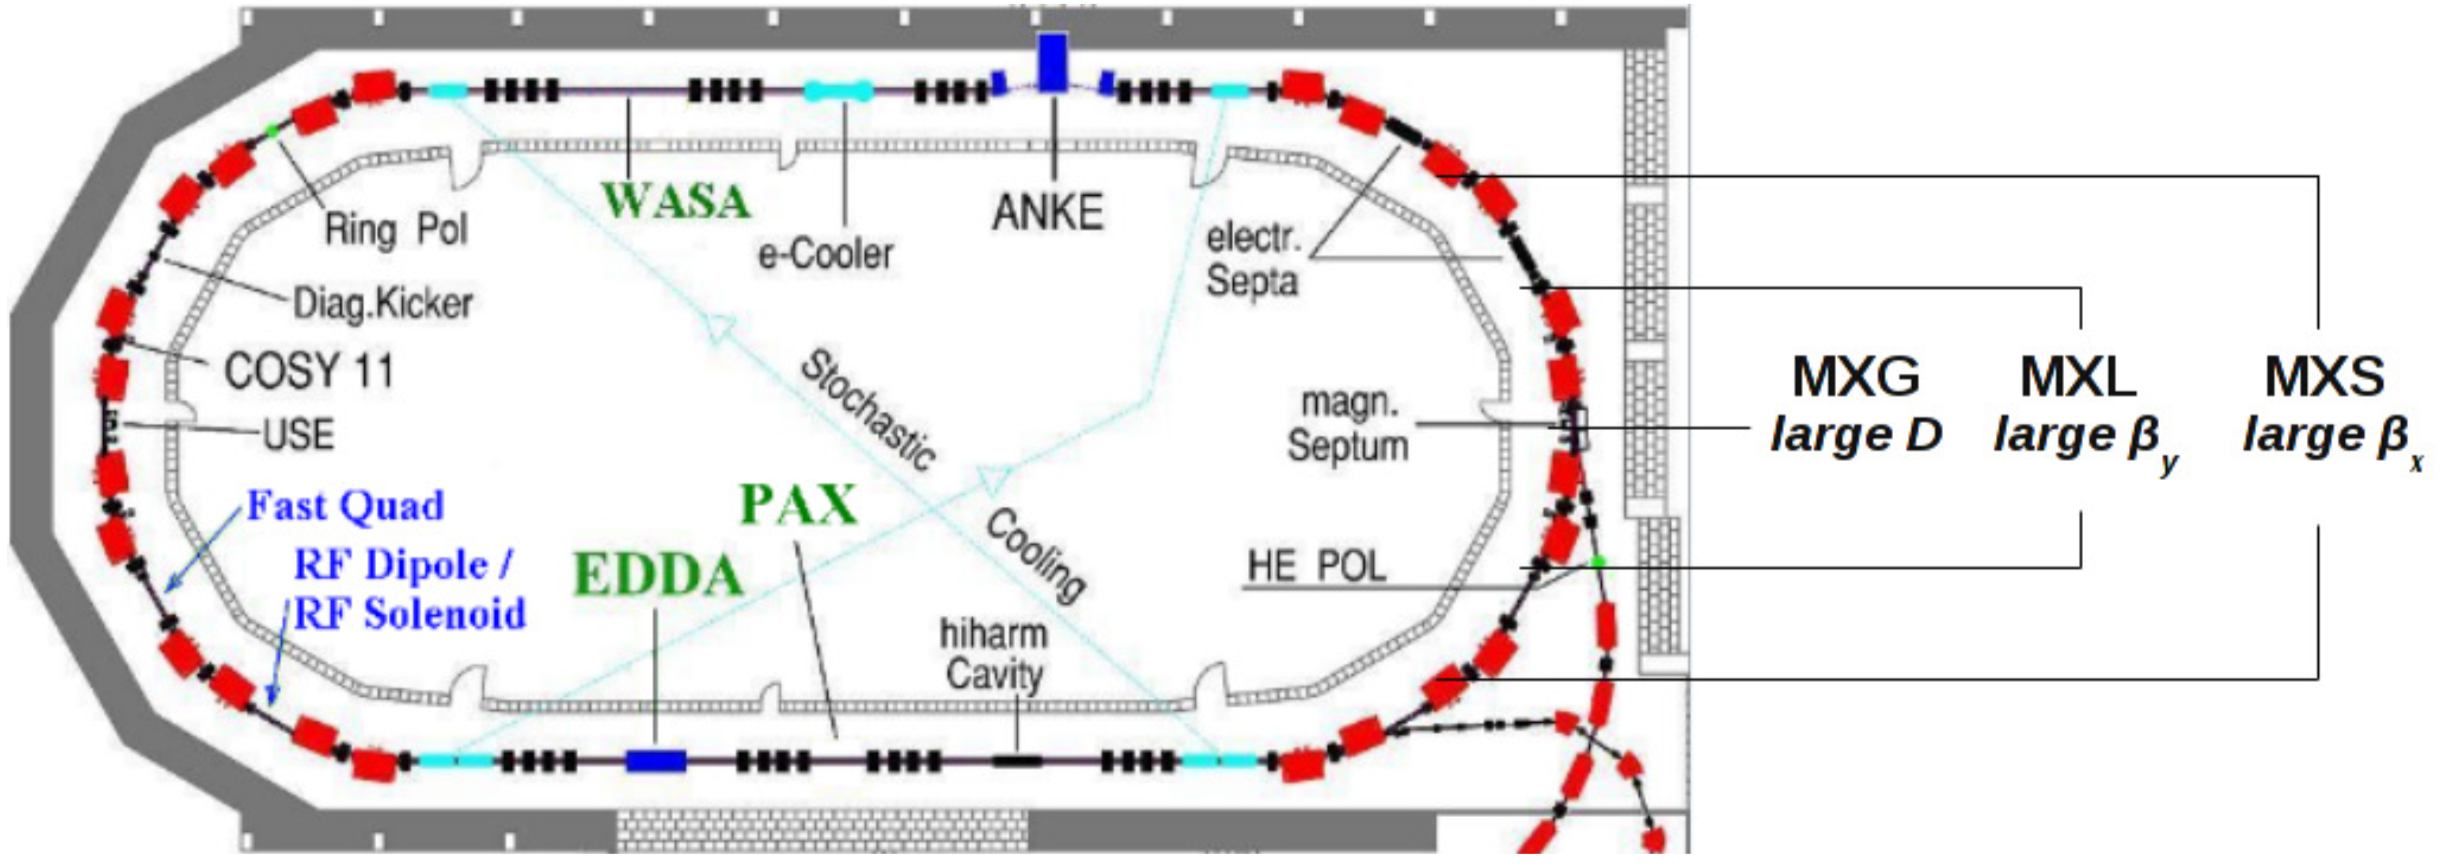
\includegraphics[width=.9\linewidth]{chapter4/COSY-sextupoles}};
	\pause
	\node (imgA) at (COSY.north east) [xshift=-3cm] {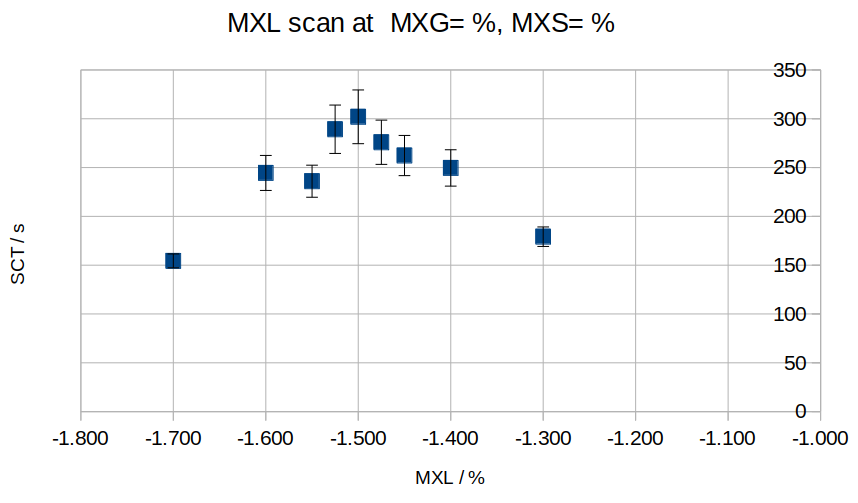
\includegraphics[width=.6\linewidth]{chapter4/SCT-April-2019/MXL_scan}};
	\pause
	\node (imgB) at (COSY.south west) [xshift=3cm, yshift=1cm] {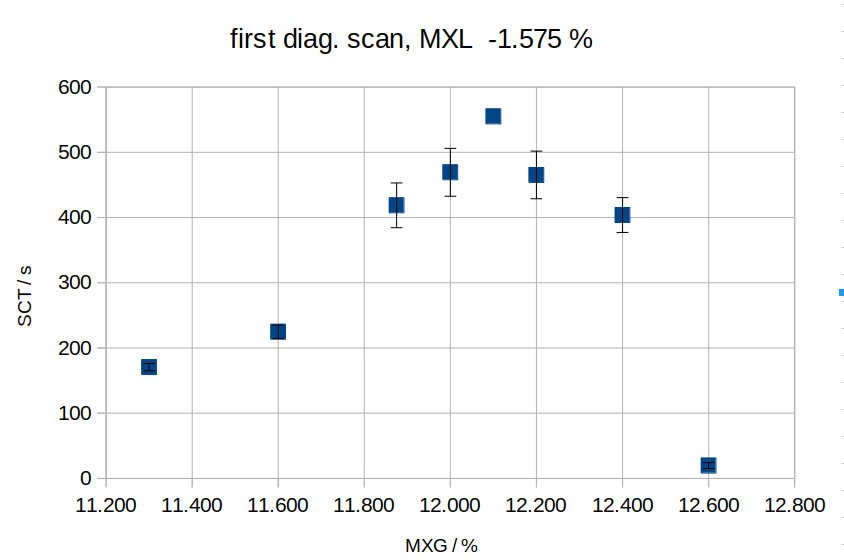
\includegraphics[width=.6\linewidth]{chapter4/SCT-April-2019/MXG_scan}};
	\end{tikzpicture}
\end{frame}


\section{Формальные вещи}
%%%%%%%%%%%%%%%%%%%%%%%%%%%%%%%%%%%%%%%%%%%%%%%%%%%%%%%%%%%%%%%%%%%%%%%%%%%%%%%%%%%%%%%%%%%%%%%%%%%%%%%%%%%
\begin{frame}{Результаты работы}
	\begin{enumerate}
		\item Разработан метод измерения ЭДМ дейтрона, основанный исключительно на измерении частоты прецессии спина частицы 
		при движении в накопительном кольце.
		\item Предложен принцип построения магнитооптической структуры кольца-накопителя для поиска ЭДМ дейтрона.
		\item Получены результаты исследования спин-декогеренции пучка дейтронов в окрестности 
		состояния ``замороженного спина.''
	\end{enumerate}
\end{frame}
\begin{frame}
	\begin{enumerate}\setcounter{enumi}{3}
		\item Исследовано влияние различного рода несовершенств элементов накопительного кольца 
		на спин-орбитальную динамику пучка.
		\item Проведено численное моделирование процедуры калибровки нормализованной частоты прецессии спина. 
		\item Проведена оценка статистических свойств разработанного метода измерения ЭДМ.
	\end{enumerate}
\end{frame}
\begin{frame}{Положения выносимые на защиту}
	\begin{enumerate}
		\item Метод измерения электрического дипольного момента дейтрона.
		\item Принцип построения магнитооптической структуры накопительного кольца.
		\item Результаты исследования спин-декогеренции пучка дейтронов в окрестности состояния ``замороженного'' спина.
		\item Результаты исследования влияния различного рода несовершенств элементов накопительного кольца 
		на спин-орбитальную динамику пучка. 
	\end{enumerate}
\end{frame}
\begin{frame}
	\begin{enumerate}\setcounter{enumi}{3}
		\item Метод калибровки нормализованной частоты прецессии спина.
		\item Результаты исследования систематических ошибок в различных методах поиска ЭДМ. 
		\item Результаты исследования статистических свойств разработанного метода.
	\end{enumerate}
\end{frame}

\begin{frame}
\begin{center}
Спасибо за внимание!
\end{center}
\end{frame}

\section{Reserve}
\begin{frame}{Возмущения спин-динамики}\centering
\begin{tikzpicture}
\node(NBAR) {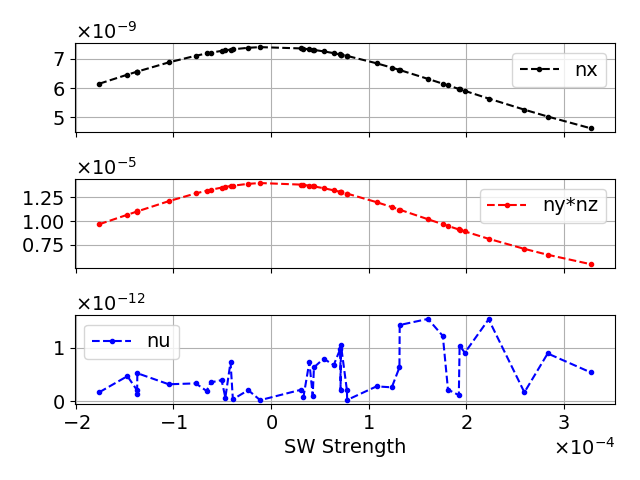
\includegraphics[width=.8\linewidth]{smp_sim/NBAR_variation_sd_vs_SW}};
\pause
\node (resid) at (NBAR.center)[xshift=2cm, yshift=-2cm] {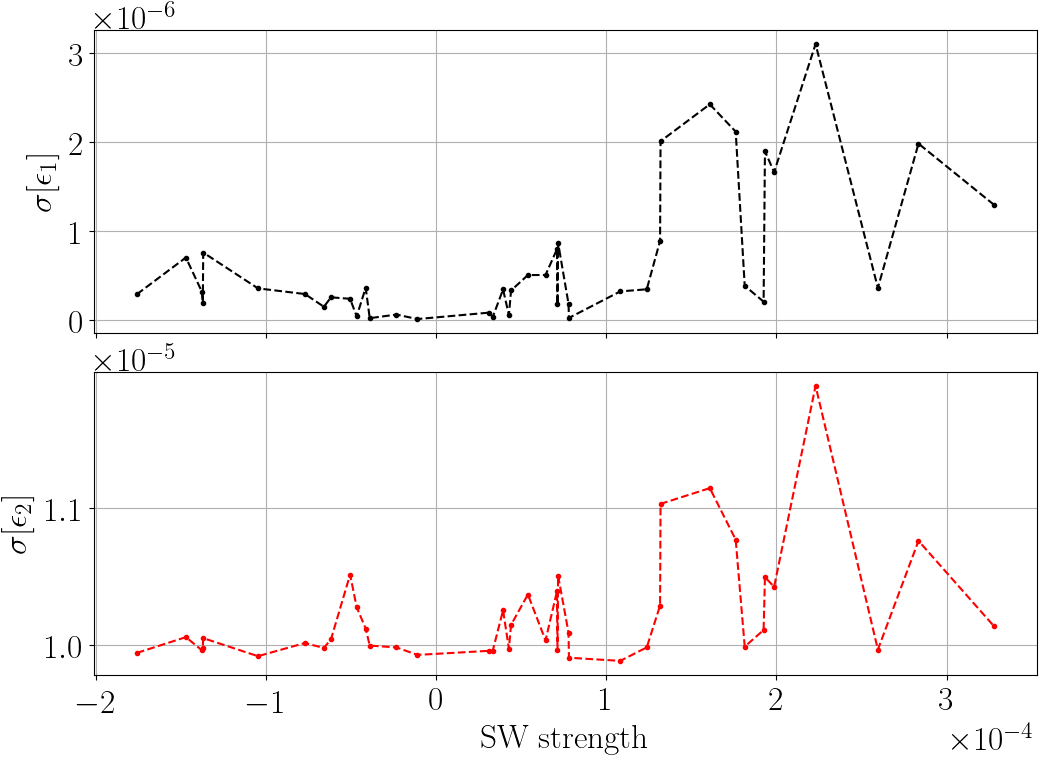
\includegraphics[width=.7\linewidth]{smp_sim/residual_SD_vs_SW(both)}};
\end{tikzpicture}
\end{frame}
\begin{frame}{Спин-декогеренция}
	\framesubtitle{Идеальная структура}
	\centering
	\begin{tikzpicture}
	\node (X) {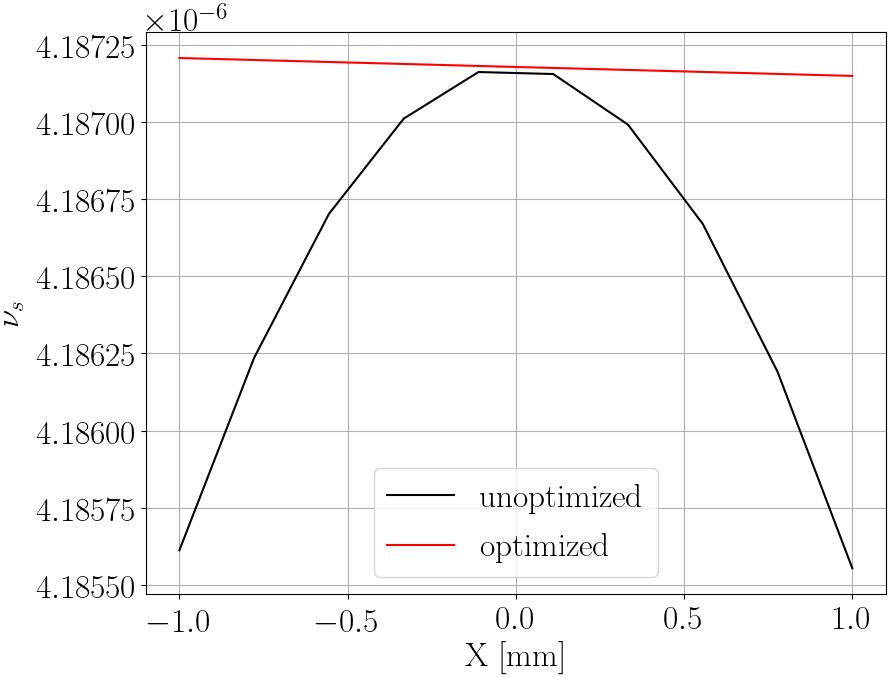
\includegraphics[height=.5\paperheight]{decoh_sim/spin_tune_decoh_x_offset}};
	\pause
	\node (Y) at (X.east)[yshift=-1.7cm]{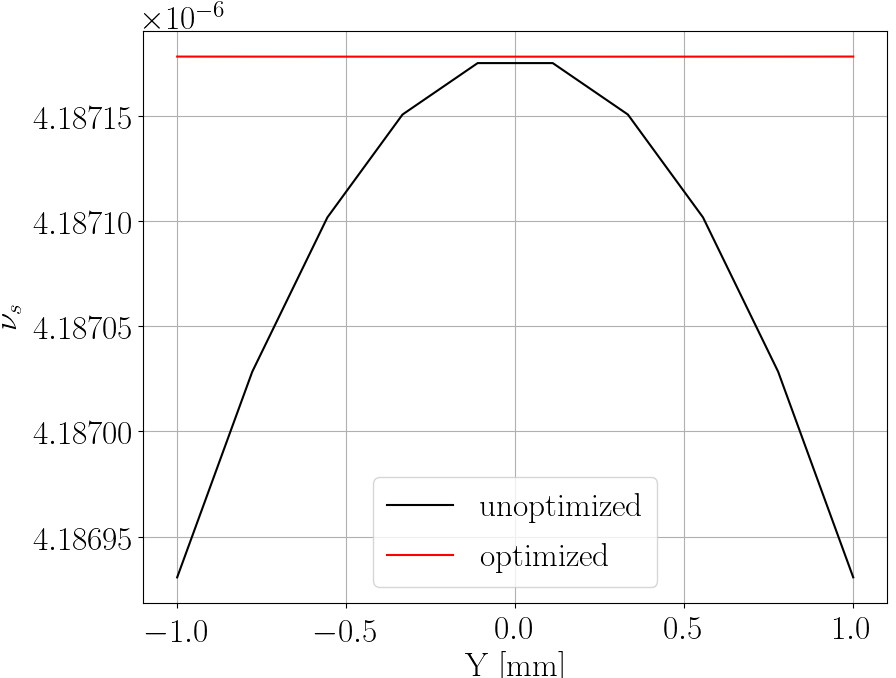
\includegraphics[height=.5\paperheight]{decoh_sim/spin_tune_decoh_y_offset}};
	\pause
	\node (D) at (X.center)[yshift=-2.3cm]{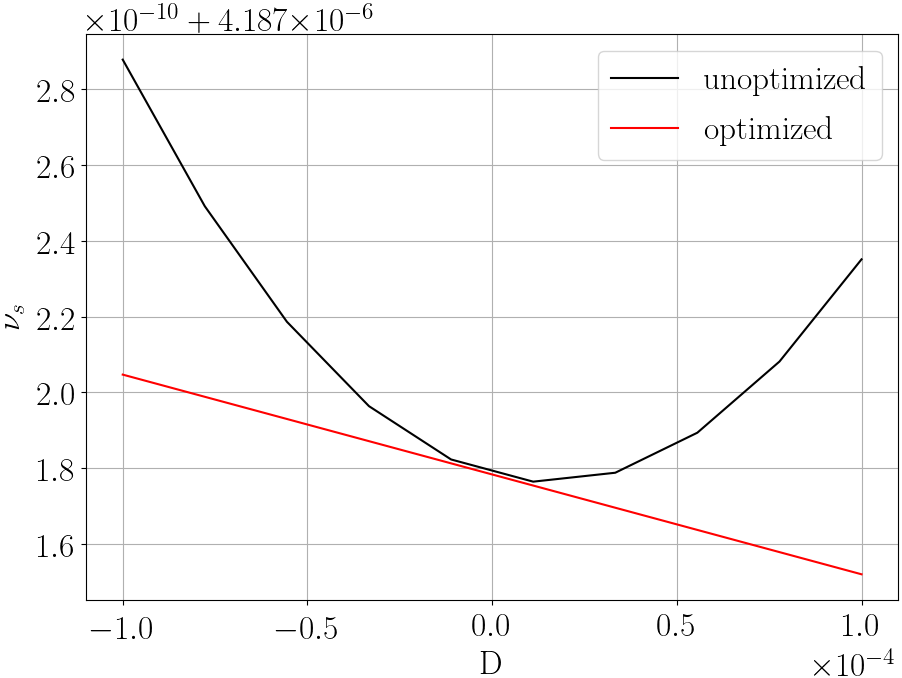
\includegraphics[height=.5\paperheight]{decoh_sim/spin_tune_decoh_d_offset}};
	\end{tikzpicture}
\end{frame}
\begin{frame}{Спин-декогеренция}
	\framesubtitle{Неидеальная структура: без секступолей}
\begin{tikzpicture}
\node (imgX) {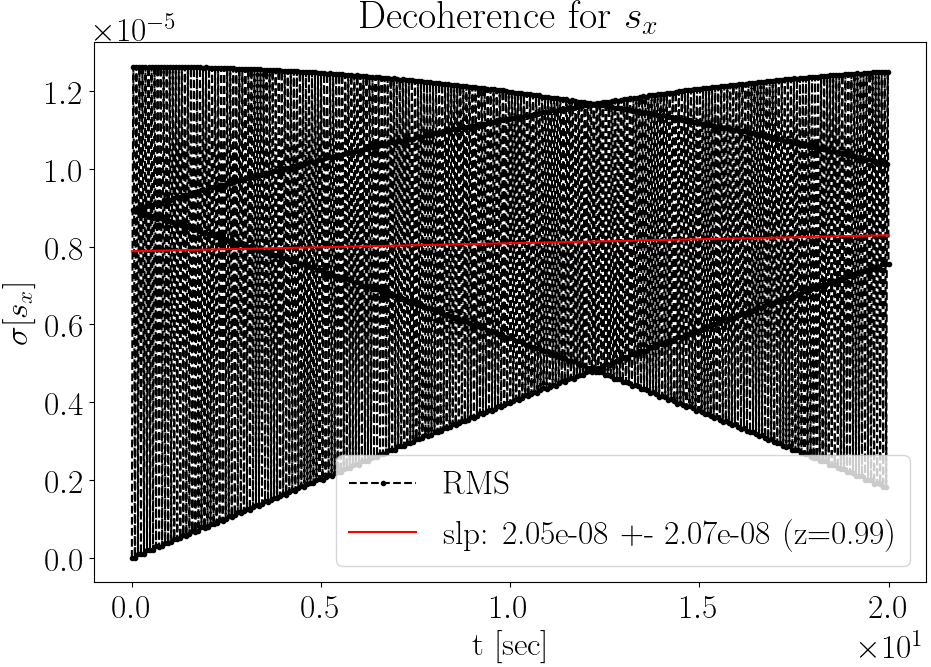
\includegraphics[width=.65\linewidth]{decoh_sim/SX_decoh_20sec_unopt}};
\pause
\node (imgY) at (imgX.south east)[yshift=1cm]{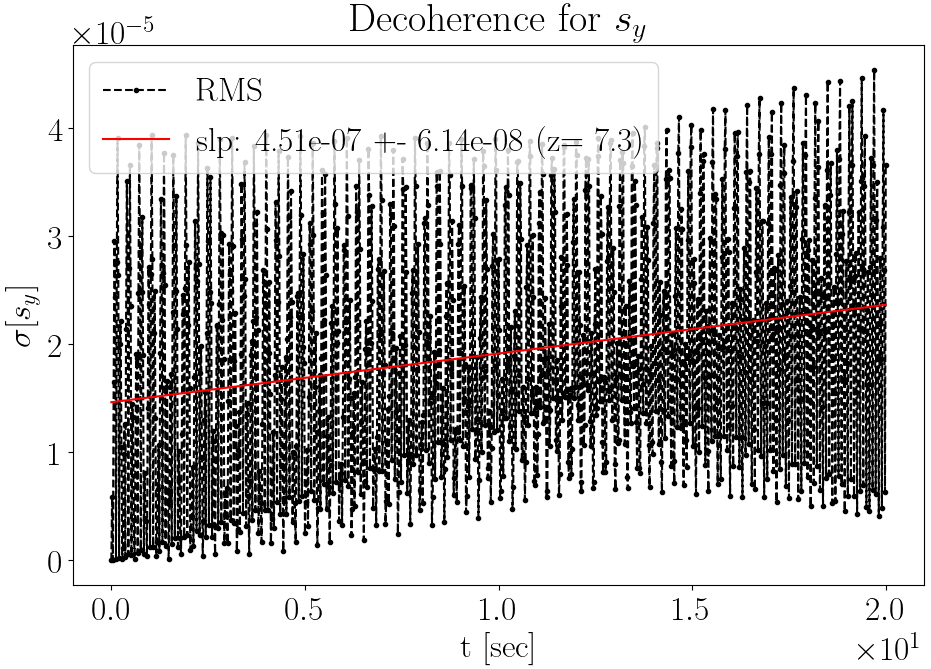
\includegraphics[width=.65\linewidth]{decoh_sim/SY_decoh_20sec_unopt}};
\end{tikzpicture}
\end{frame}
\begin{frame}{Спин-декогеренция}
	\framesubtitle{Неидеальная структура: с секступолями}
\begin{tikzpicture}
\node (imgX) {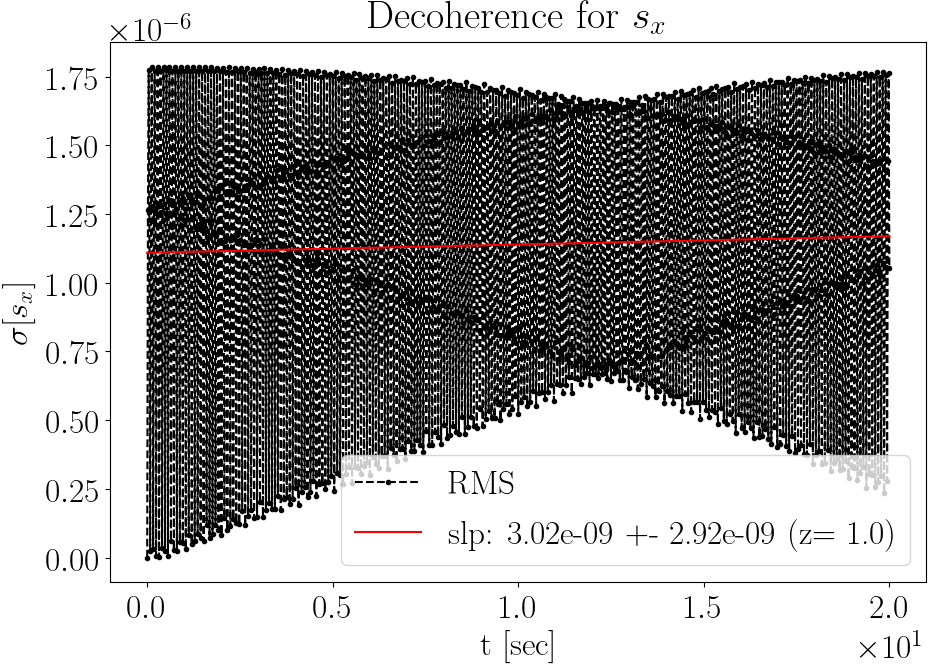
\includegraphics[width=.65\linewidth]{decoh_sim/SX_decoh_20sec_opt}};
\pause
\node (imgY) at (imgX.south east)[yshift=1cm]{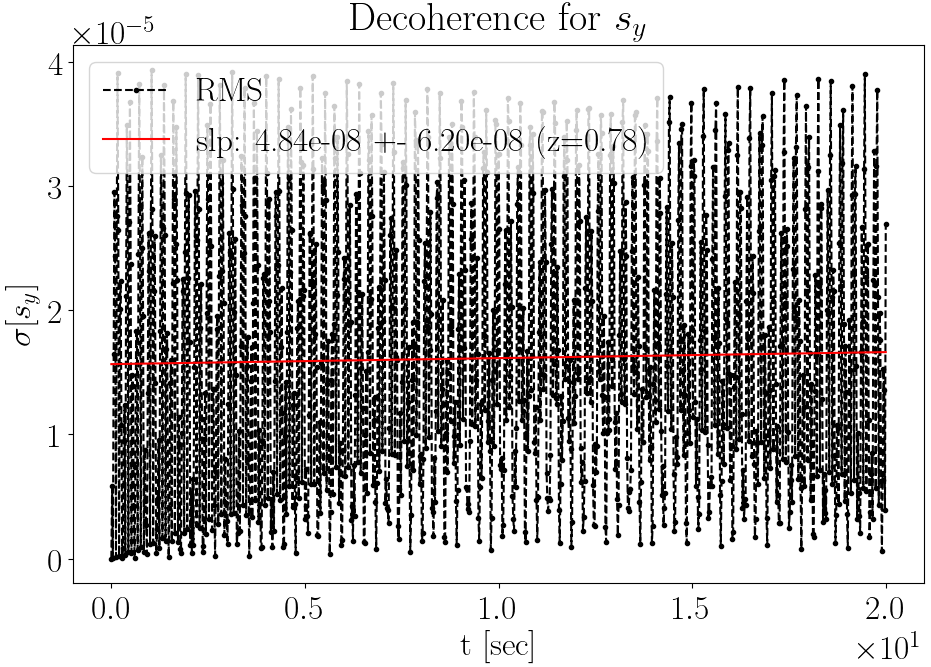
\includegraphics[width=.65\linewidth]{decoh_sim/SY_decoh_20sec_opt}};
\end{tikzpicture}
\end{frame}
\begin{frame}{Спин-декогеренция}\centering
	\framesubtitle{Выравнивание осей стабильного спина частиц}
	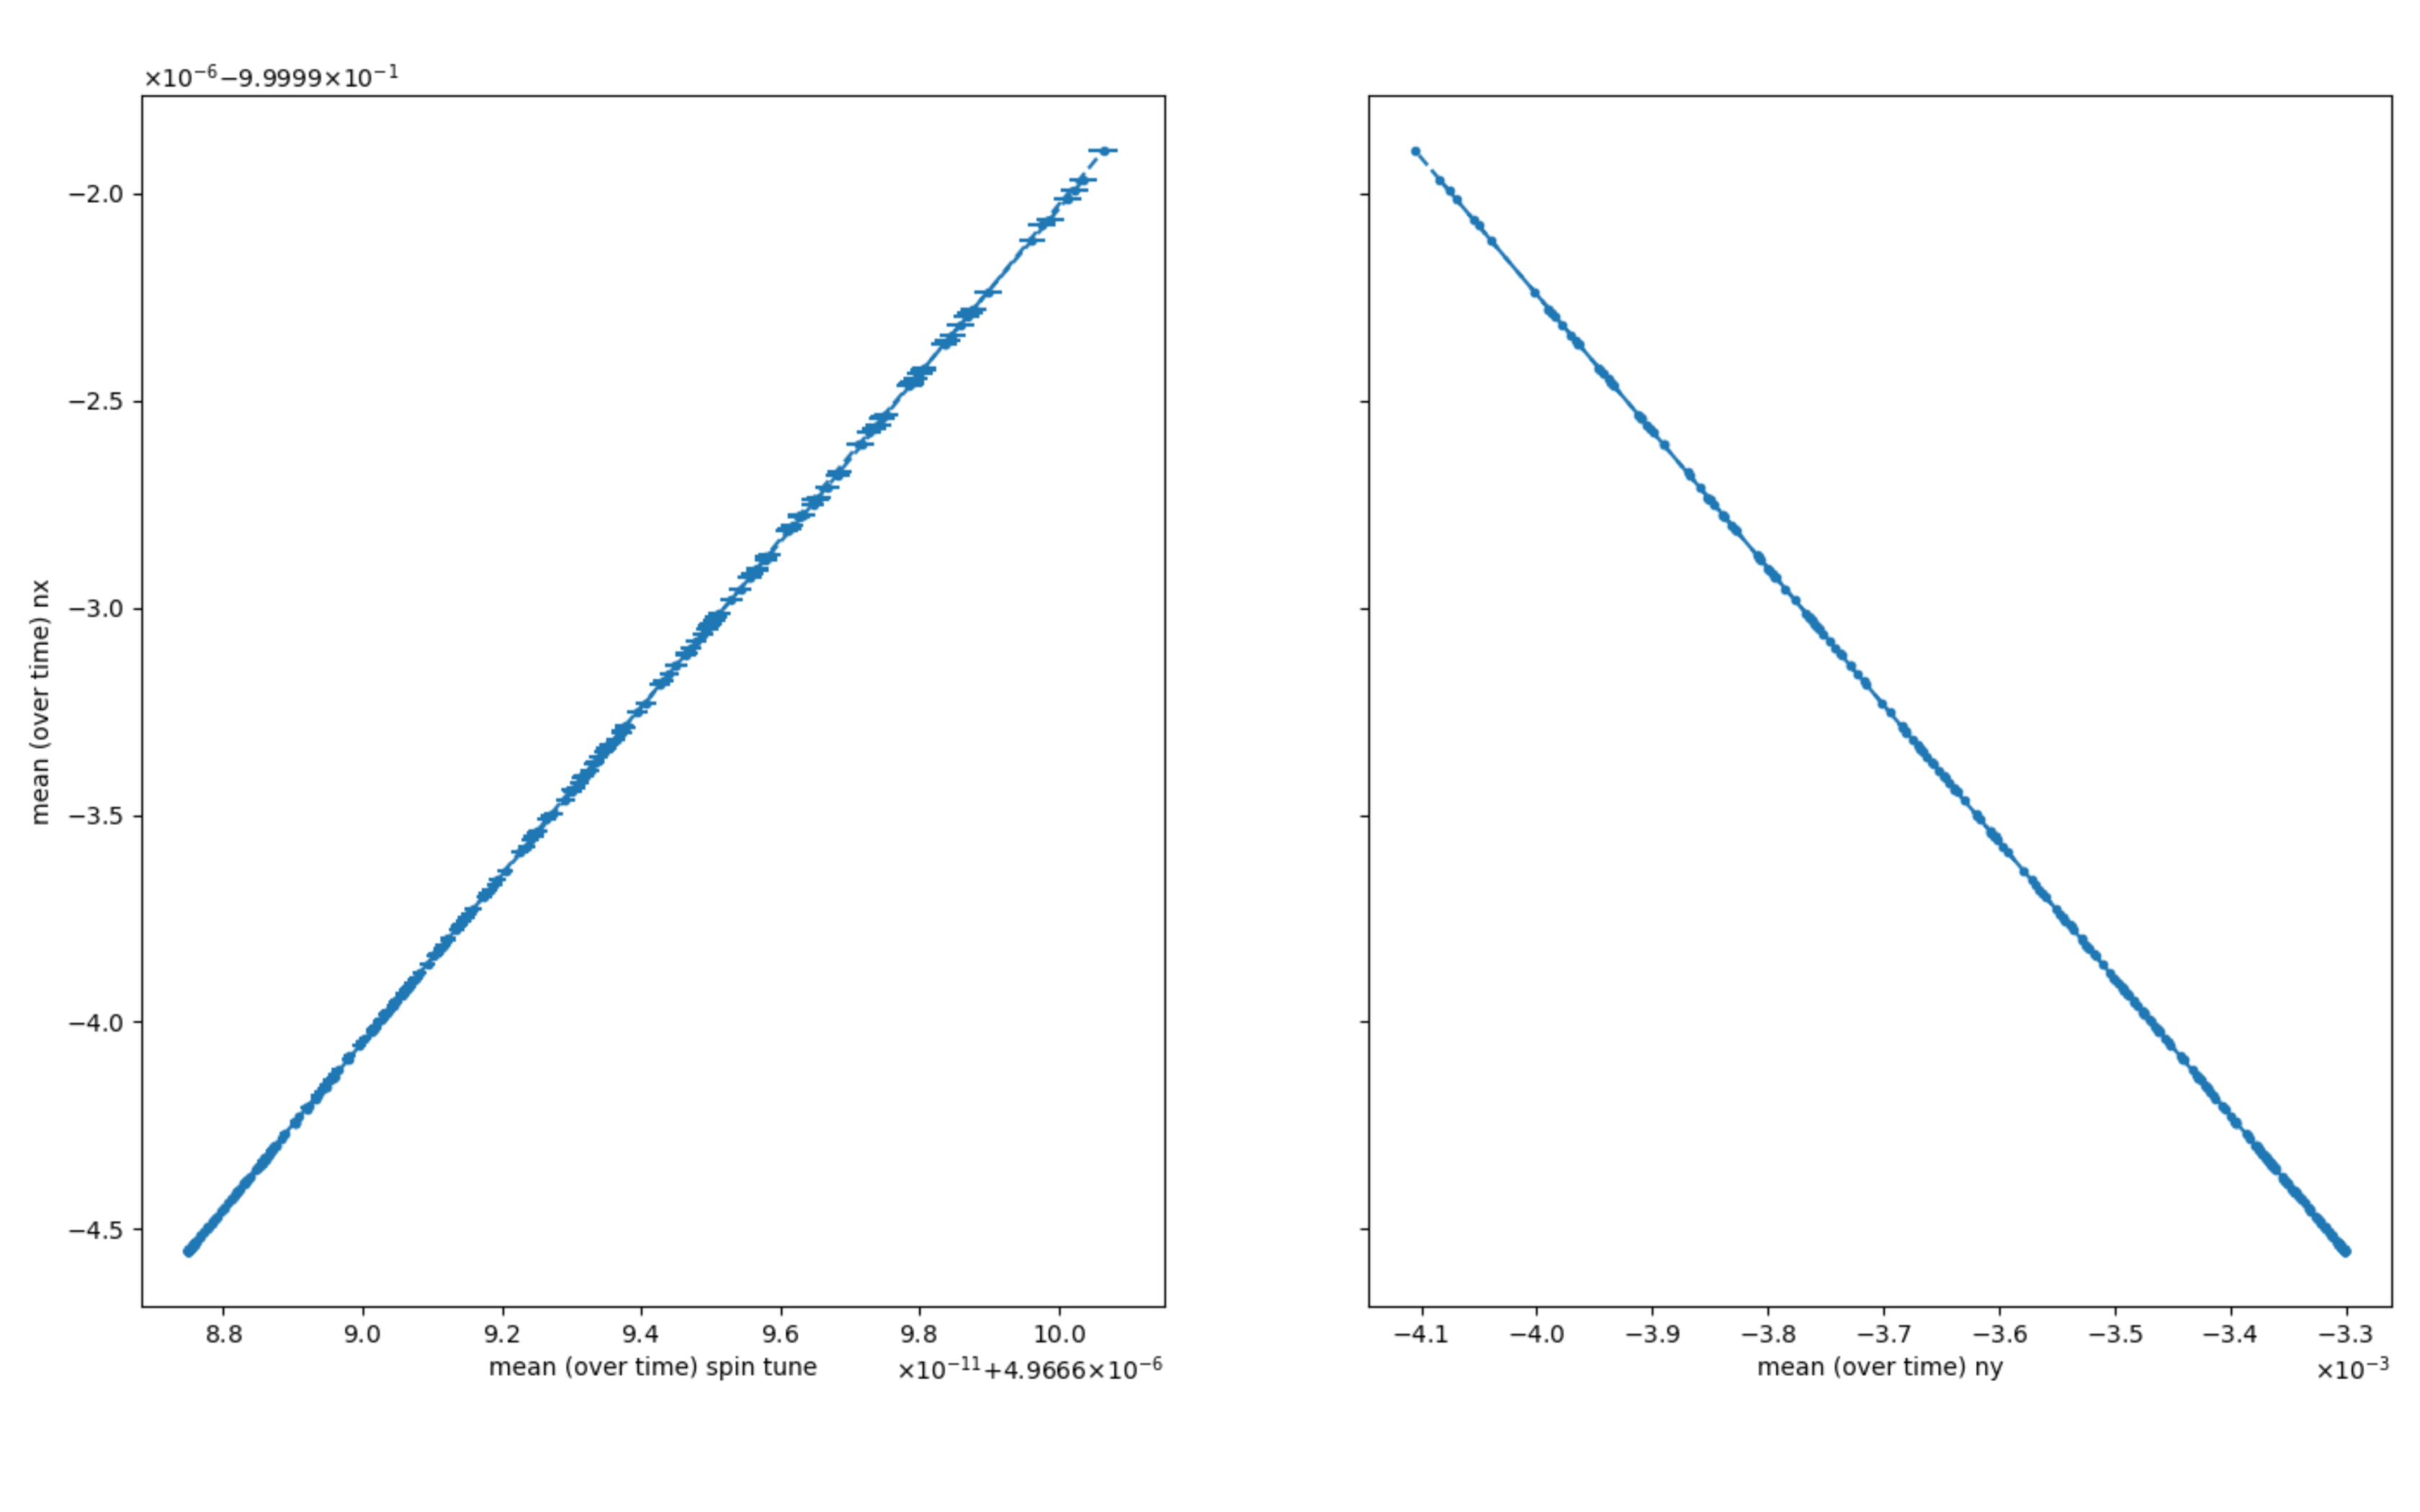
\includegraphics[width=.9\linewidth]{decoh_sim/mean_n_bar_vs_spin_tune}
\end{frame}
\begin{frame}{МДМ-компонента спин-прецессии}
	\centering
	\begin{tikzpicture}
	\node (A) {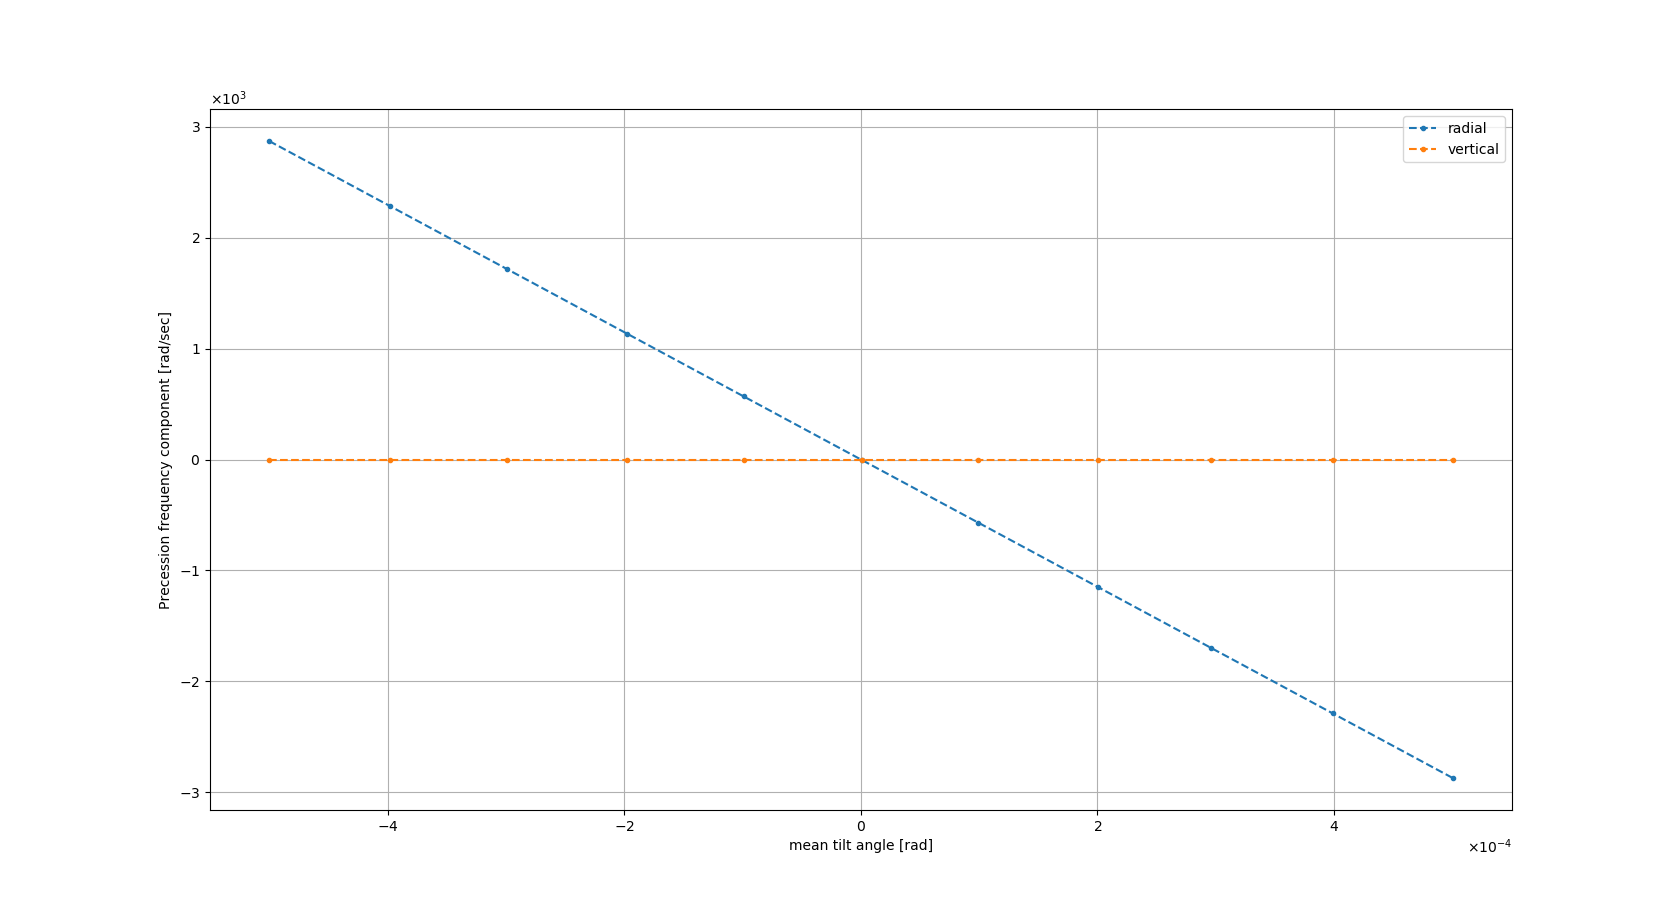
\includegraphics[width=.7\linewidth]{fake_signal_sim/linearity_test_shifting_gauss_freq}};
	\pause
	\node (B) at (A.center)[xshift=2cm, yshift=-2cm]  {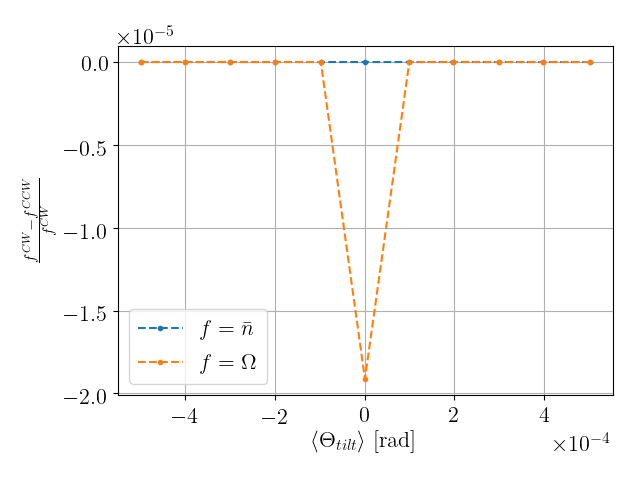
\includegraphics[width=.7\linewidth]{fake_signal_sim/linearity_test_shifting_gauss_rel_diff}};
	\end{tikzpicture}
\end{frame}
\begin{frame}{Калибровка МДМ-сигнала}
	\framesubtitle{Почему это важно?}
	\begin{block}{ЭДМ-статистика}
		\begin{align*}
		\hat\w_{edm} &= \frac12(\hat\w_x^+ + \hat\w_x^-) \\
		&= \w_{edm} + \underbrace{\frac{1}{\sqrt2}\sigma_{\hat\w}}_{stat} + \underbrace{(\w_{mdm}^+ - \w_{mdm}^-)}_{syst}
		\end{align*}
	\end{block}
	\begin{block}{Утверждение}
		$\left[\w_y^{mdm+} - \w_y^{mdm-} \to 0\right] \Rightarrow \left[\w_x^{mdm+} - \w_x^{mdm-} \to 0\right]$
	\end{block}
\end{frame}
\begin{frame}{Калибровка МДМ-сигнала}
	\framesubtitle{Калибровочный график}
	\centering
	\begin{tikzpicture}
	%\node (A) {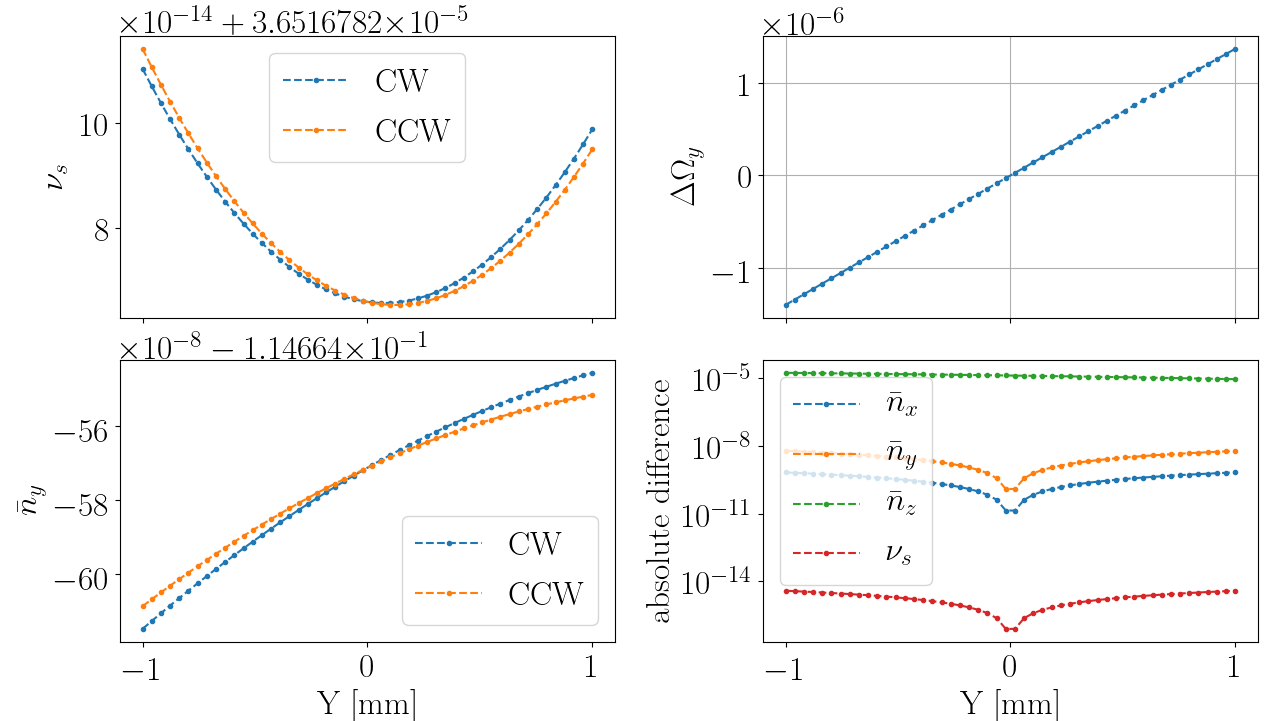
\includegraphics[width=\linewidth]{GFF/GFF_stune_range_Y}};
	%\pause
	\node (B)  {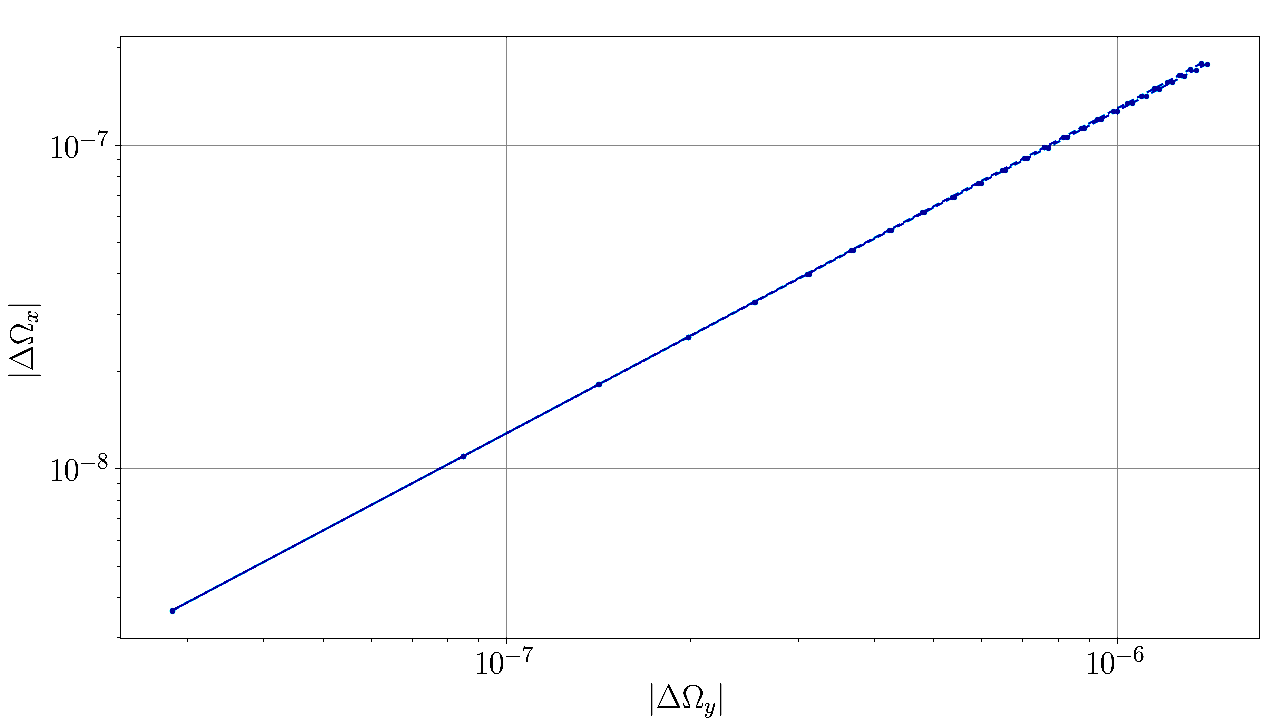
\includegraphics[width=\linewidth]{GFF/GFF_omegas_range_Y}};
	\end{tikzpicture}
\end{frame}

\begin{frame}{Статистическое моделирование}
	\framesubtitle{Модулированная схема выборки}
	\begin{figure}[H]\centering
%		\begin{minipage}{.6\linewidth}
			\begin{tikzpicture}
			\begin{axis}[axis lines=center, xlabel=$t$, domain=-.5:2*pi, legend pos=outer north east, width=.8\linewidth,
			scatter/use mapped color={draw=black, fill=black}
			]
			\addplot[color=blue, name path=signal, domain=-.1:2*pi,samples=50] {sin(deg(x))};
			\draw[dashed] (axis cs:.785,0) -- (axis cs:.785,{sin(deg(.785))});
			\draw[dashed] (axis cs:2.36,0) -- (axis cs:2.36,{sin(deg(2.36))});
			\draw[dashed] (axis cs:3.93,0) -- (axis cs:3.93,{sin(deg(3.93))});
			\draw[dashed] (axis cs:5.5,0) -- (axis cs:5.5,{sin(deg(5.5))});
			\path[name path=axis] (axis cs:0,0) -- (axis cs:2*pi,0);
			\addplot[fill=blue, opacity=.05] fill between [of=signal and axis, soft clip={domain=0:.785}];
			\addplot[fill=blue, opacity=.05] fill between [of=signal and axis, soft clip={domain=2.36:3.93}];
			\addplot[fill=blue, opacity=.05] fill between [of=signal and axis, soft clip={domain=5.5:2*pi}];
			\addplot [scatter, only marks, domain=-.1:.7, samples=5] {sin(deg(x))};
			\addplot [scatter, only marks, domain=2.4:3.9, samples=10, mark=*] {sin(deg(x))};
			\addplot [scatter, only marks, domain=5.6:6.2, samples=5, mark=*] {sin(deg(x))};
			\end{axis}     
			\end{tikzpicture}
%		\end{minipage}%
%		\begin{minipage}{.4\linewidth}
%			\caption{Частотно-модулированная выборка: измерения делаются только в максимально информативных точках,
%				находящихся в окрестностях узлов сигнала\label{fig:modulated_sampling}}
%		\end{minipage}
	\end{figure}
\end{frame}

%\begin{frame}[allowframebreaks]
%	\frametitle{Основные публикации по теме диссертации}
%	\begin{thebibliography}{9}
%		\bibitem{Stats-LaPlas}
%		A.E. Aksentev, Y.V. Senichev, ``Statistical precision in charged particle {EDM} search in storage rings.'' J. Phys.: Conf. Ser. \textbf{941} 012083 (2017)
%		\bibitem{Stats-IPAC}
%		A.E. Aksentyev, Y.V. Senichev,
%		``Model of Statistical Errors in the Search for the Deuteron EDM in the Storage Ring,''
%		in \emph{Proc. IPAC'17}, Copenhagen, Denmark, May 2017, pp. 2258--2260,
%		\url{https://doi.org/10.18429/JACoW-IPAC2017-TUPVA079}.
%		\bibitem{SOD-modeling-LaPlas}
%		A. Aksentev ``Modeling of spin-orbital dynamics in a storage ring.'' J. Phys.: Conf. Ser. \textbf{1238} 012079 (2019)		
%		\bibitem{SD-LaPlas}
%		A. E. Aksentyev, Y. V. Senichev, ``Spin Decoherence in a Frozen Spin Lattice, Its Suppression and Effect on the Frequency Domain Edm Statistic,''  в процессе публикации.
%		\bibitem{GFF-IPAC}
%		A.E. Aksentyev, Y.V. Senichev, ``Simulation of the Guide Field Flipping Procedure for the Frequency Domain Method,'' in \emph{Proc. IPAC'19}, Melbourne, Australia, May 2019, pp. 858--860, \url{doi:10.18429/JACoW-IPAC2019-MOPTS010}
%		\bibitem{SMP-IPAC}
%		A.E. Aksentyev, Y.V. Senichev, ``Spin Motion Perturbation Effect on the EDM Statistic in the Frequency Domain Method,'' in \emph{Proc. IPAC'19}, Melbourne, Australia, May 2019, pp. 861--863,
%		\url{doi:10.18429/JACoW-IPAC2019-MOPTS011}
%		\bibitem{SD-IPAC}
%		A.E. Aksentyev, Y.V. Senichev, ``Spin Decoherence in the Frozen Spin Storage Ring Method of Search for a Particle EDM,'' in \emph{Proc. IPAC'19}, Melbourne, Australia, May 2019, pp. 864--866,
%		\url{doi:10.18429/JACoW-IPAC2019-MOPTS012}
%	\end{thebibliography}
%\end{frame}

\end{document} 
